I will explore here more technical details on the design and calibration explored as part of this project and necessary to extracting scientific information from the IRVB.
\section{MASTU design and implementation}\label{MASTUdesign}
The pinhole has been located off centre with respect to the foil for the field of view to point toward the X-point. The power density on the foil was simulated for stand off of three lengths (45, 60, 75 mm, see \autoref{fig:IRVB_components} for the location of this item) and pinhole diameters (4, 6, 8 mm). The results from CHERAB simulations are shown in \autoref{fig:cherab1}.


\begin{figure}
     \centering
     \begin{subfigure}{0.3\textwidth}
         \centering
         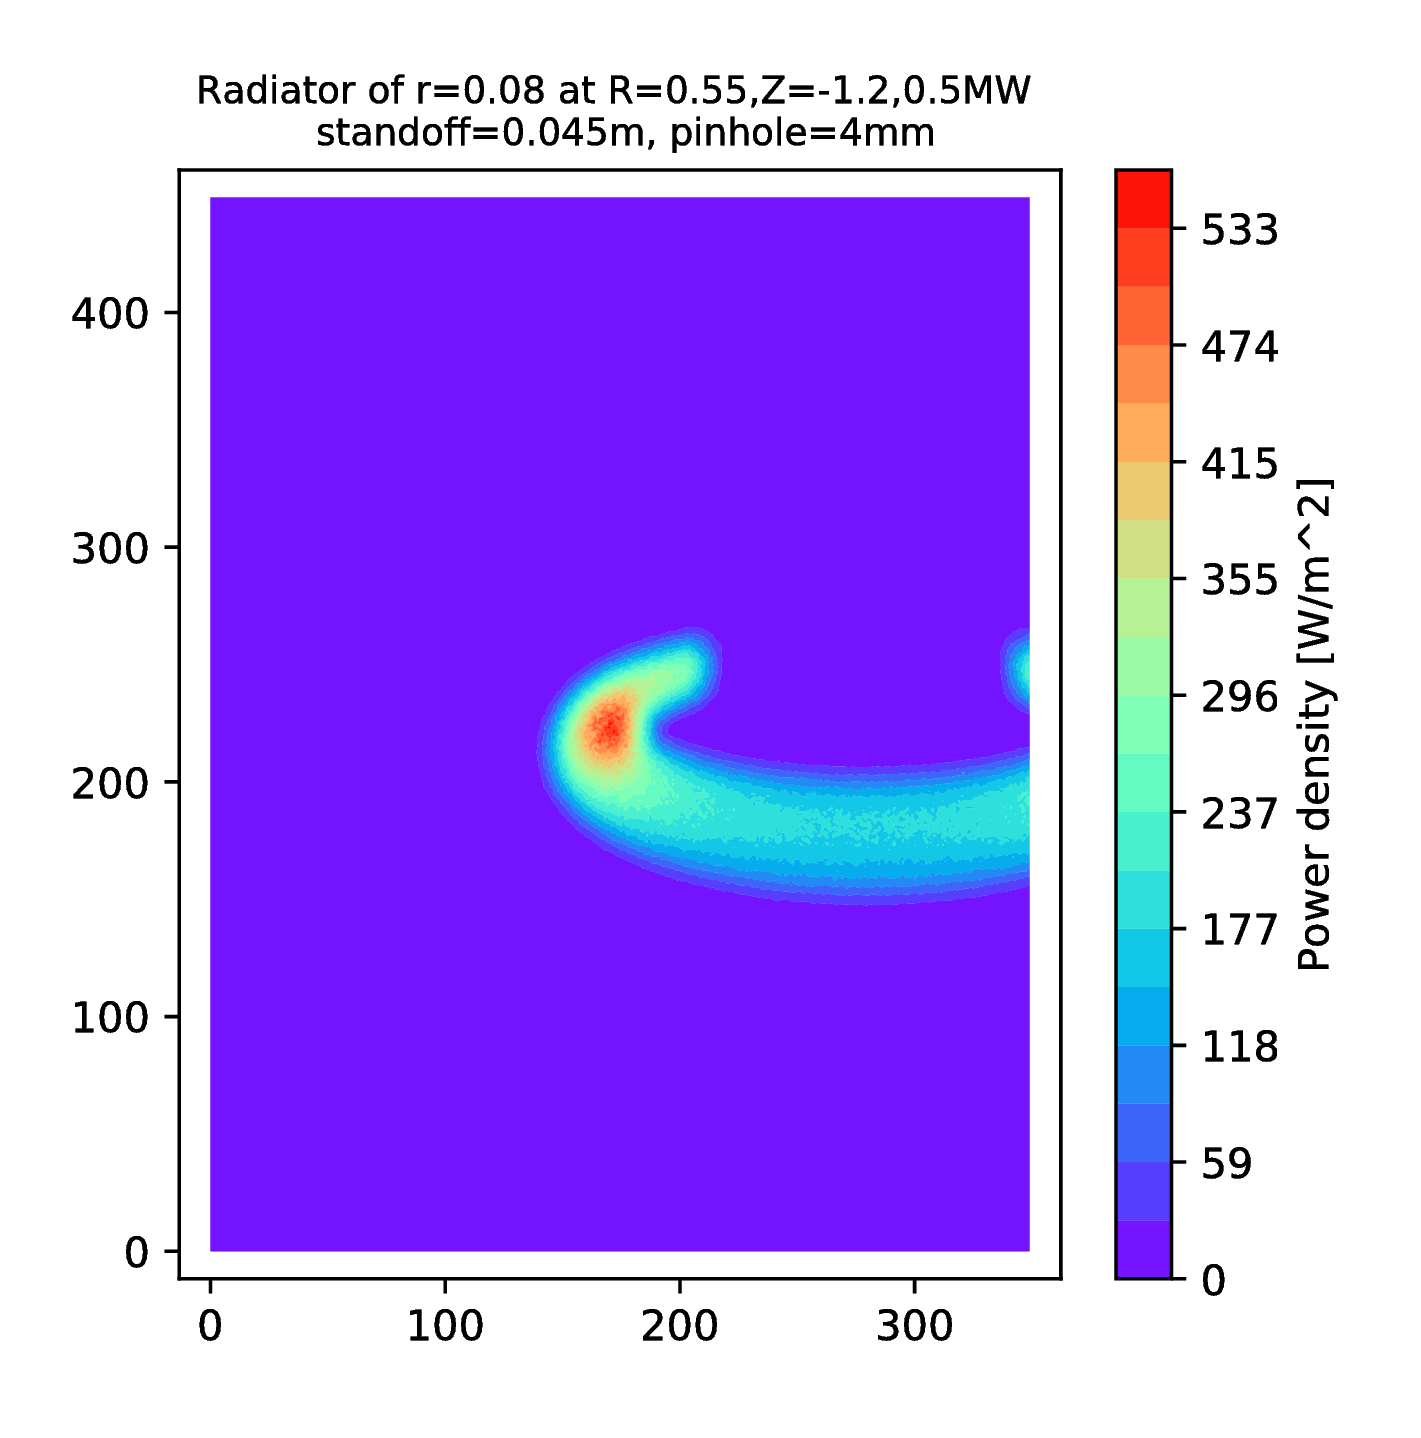
\includegraphics[trim={70 0 125 0},clip,width=\textwidth]{Chapters/appendix1/figs/4_45.png}
         \caption{pinhole 4mm/stand-off 45mm}
         \label{fig:4_45}
     \end{subfigure}
     \hfill
     \begin{subfigure}{0.3\textwidth}
         \centering
         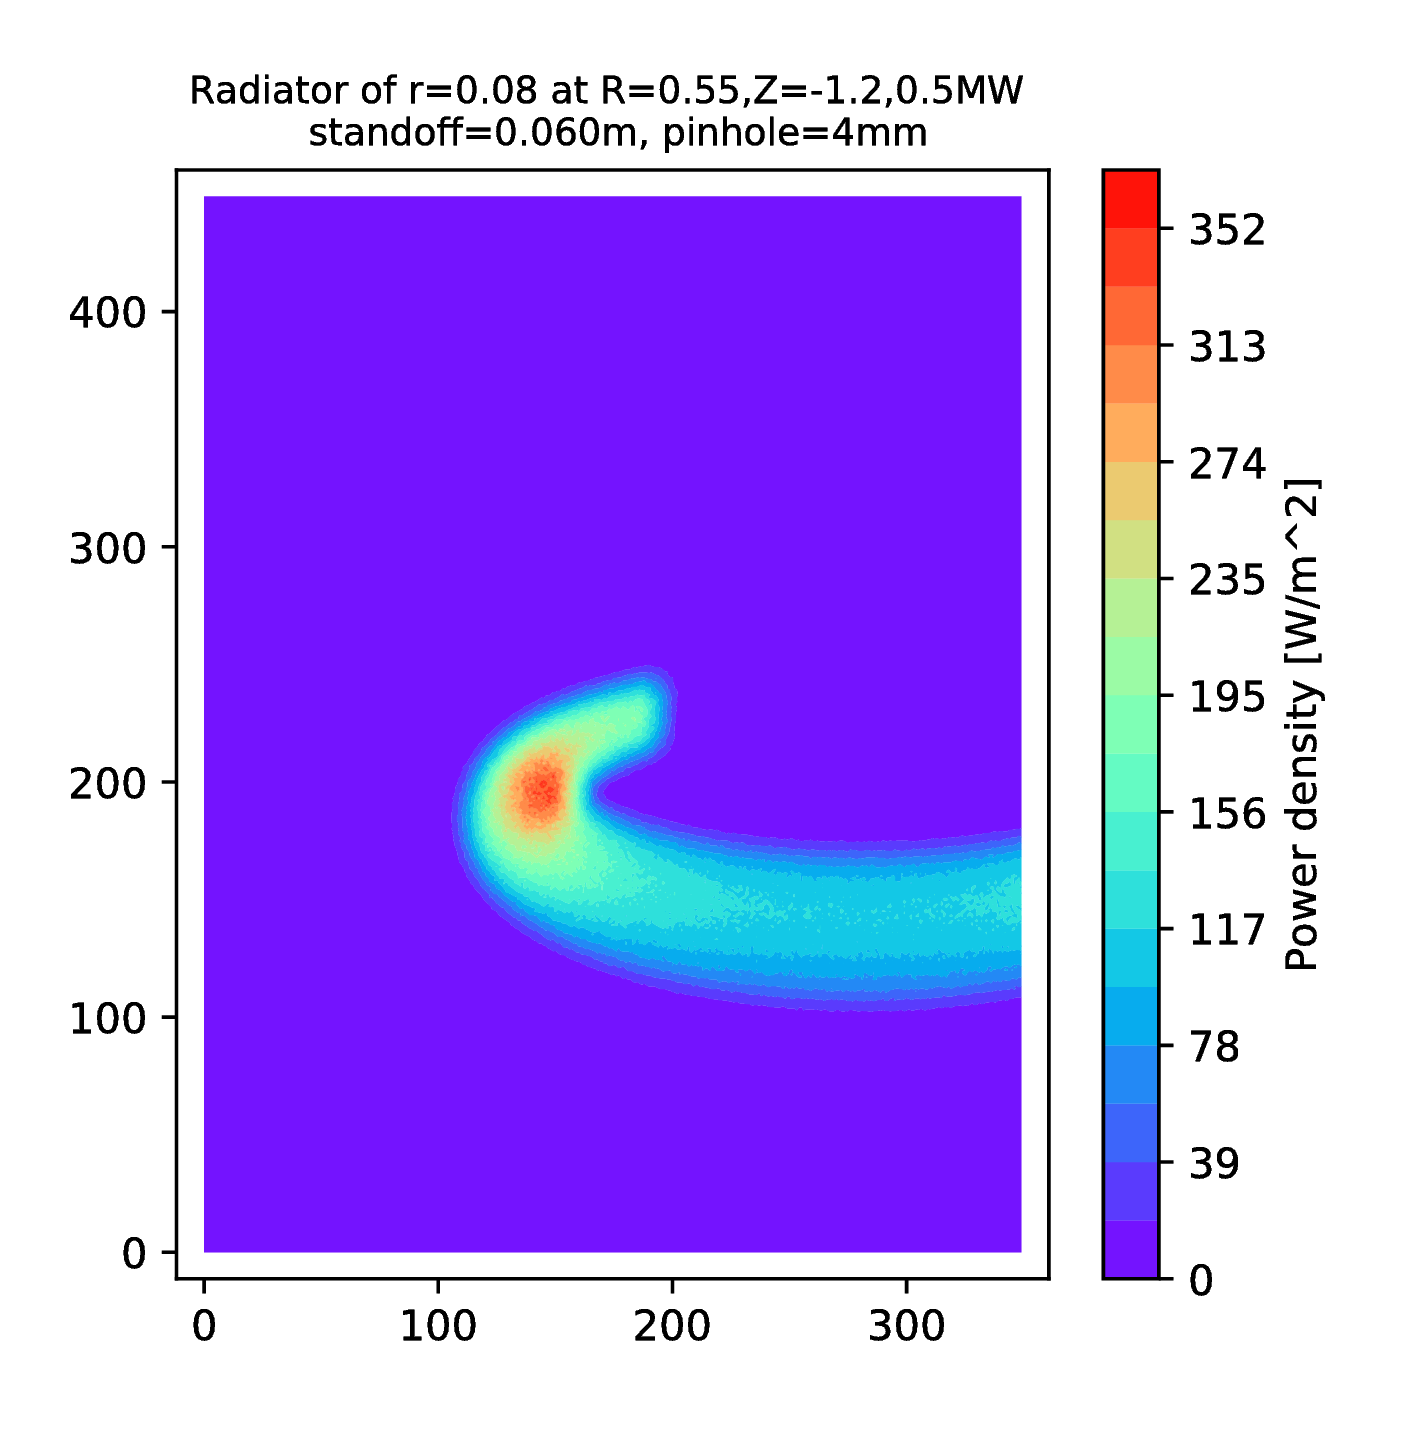
\includegraphics[trim={70 0 125 0},clip,width=\textwidth]{Chapters/appendix1/figs/4_60.png}
         \caption{$4/60$}
         \label{fig:4_60}
     \end{subfigure}
     \hfill
     \begin{subfigure}{0.325\textwidth}
         \centering
         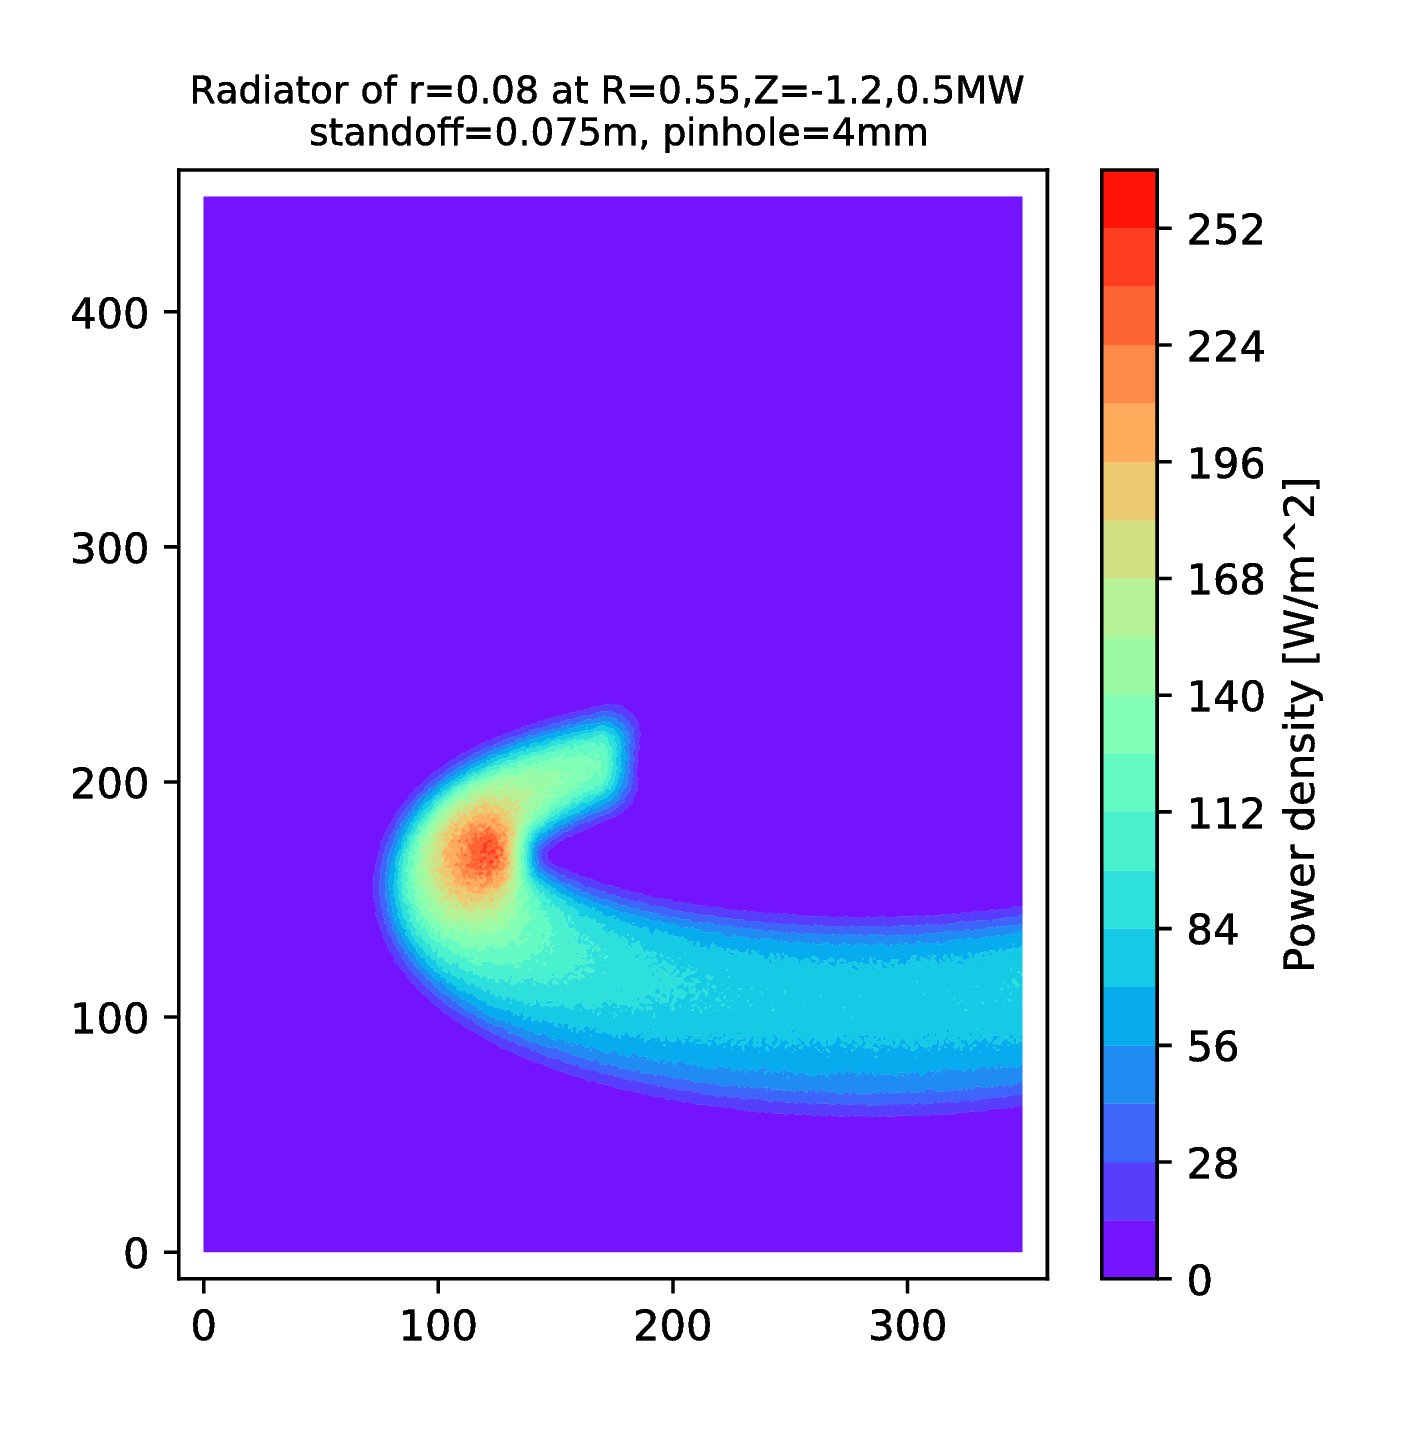
\includegraphics[trim={70 0 0 0},clip,width=\textwidth]{Chapters/appendix1/figs/4_75.png}
         \caption{$4/75$}
         \label{fig:$4_75$}
     \end{subfigure}
     \begin{subfigure}{0.3\textwidth}
         \centering
         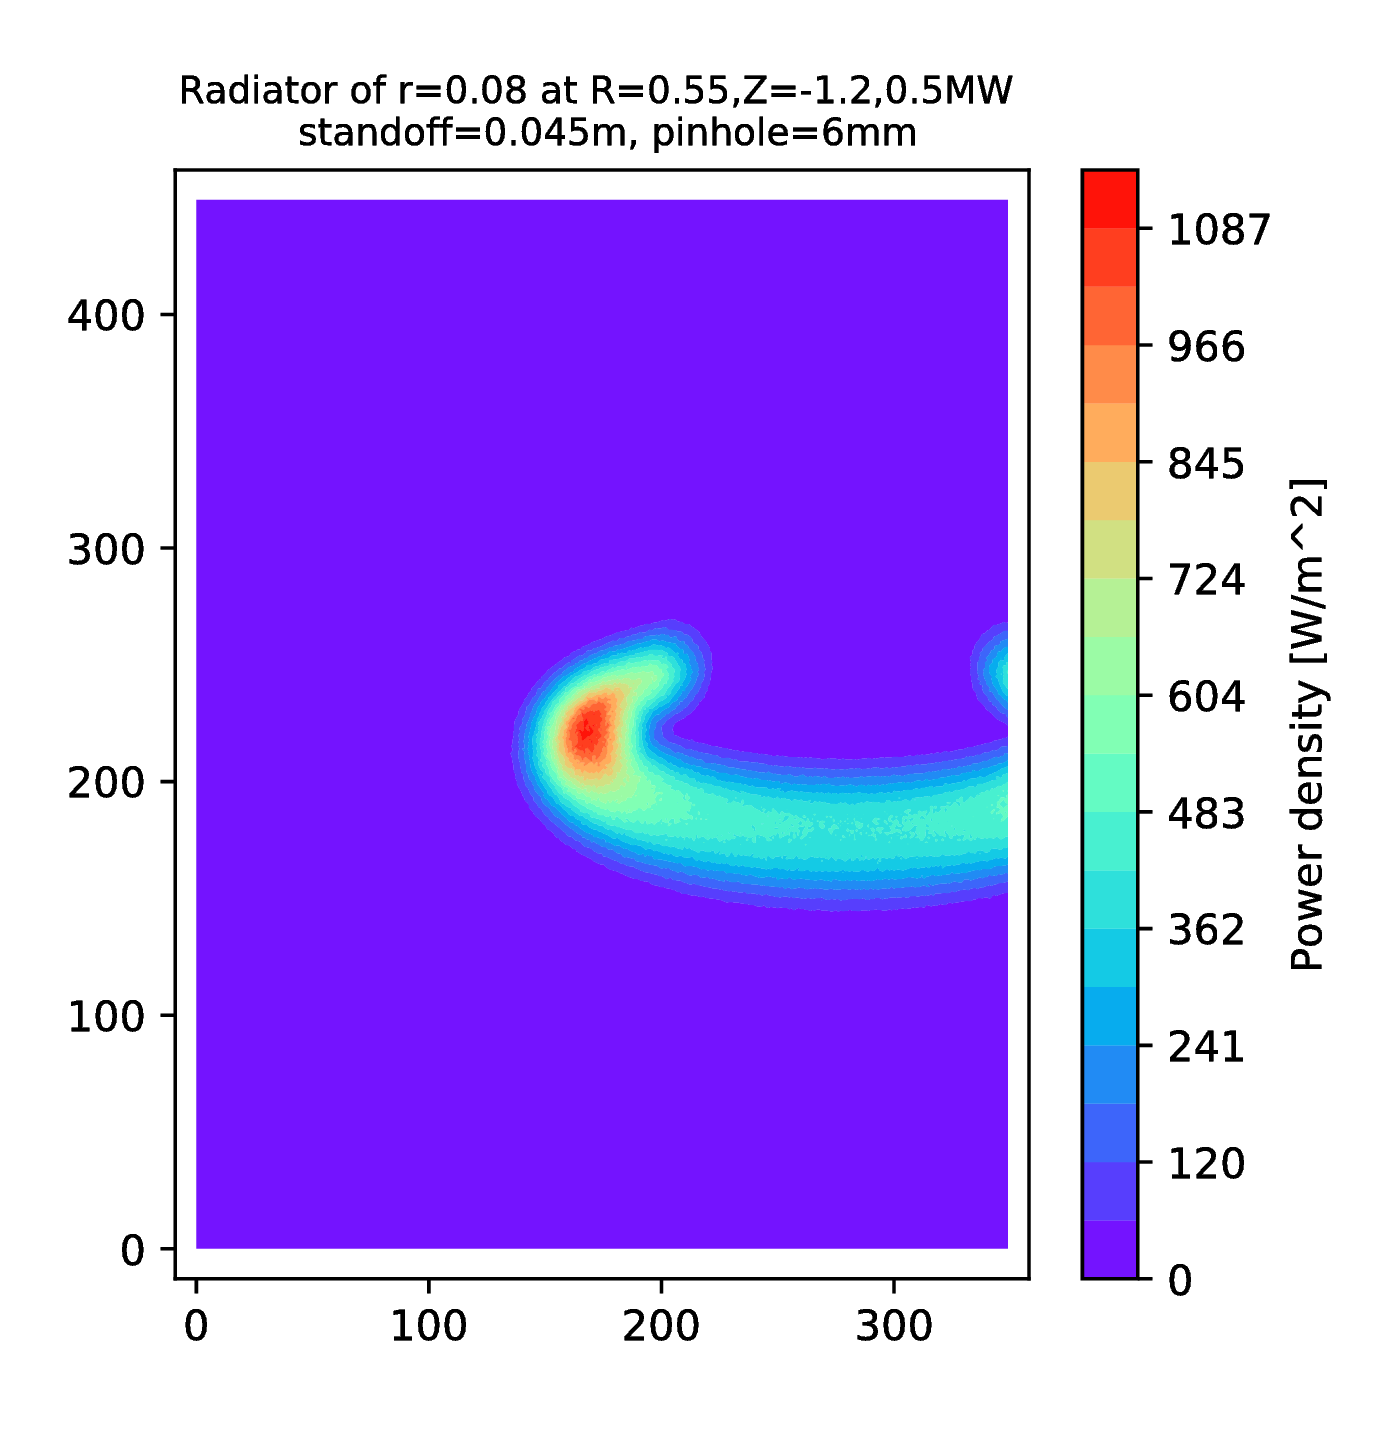
\includegraphics[trim={70 0 110 0},clip,width=\textwidth]{Chapters/appendix1/figs/6_45.png}
         \caption{$6/45$}
         \label{fig:6_45}
     \end{subfigure}
     \hfill
     \begin{subfigure}{0.3\textwidth}
         \centering
         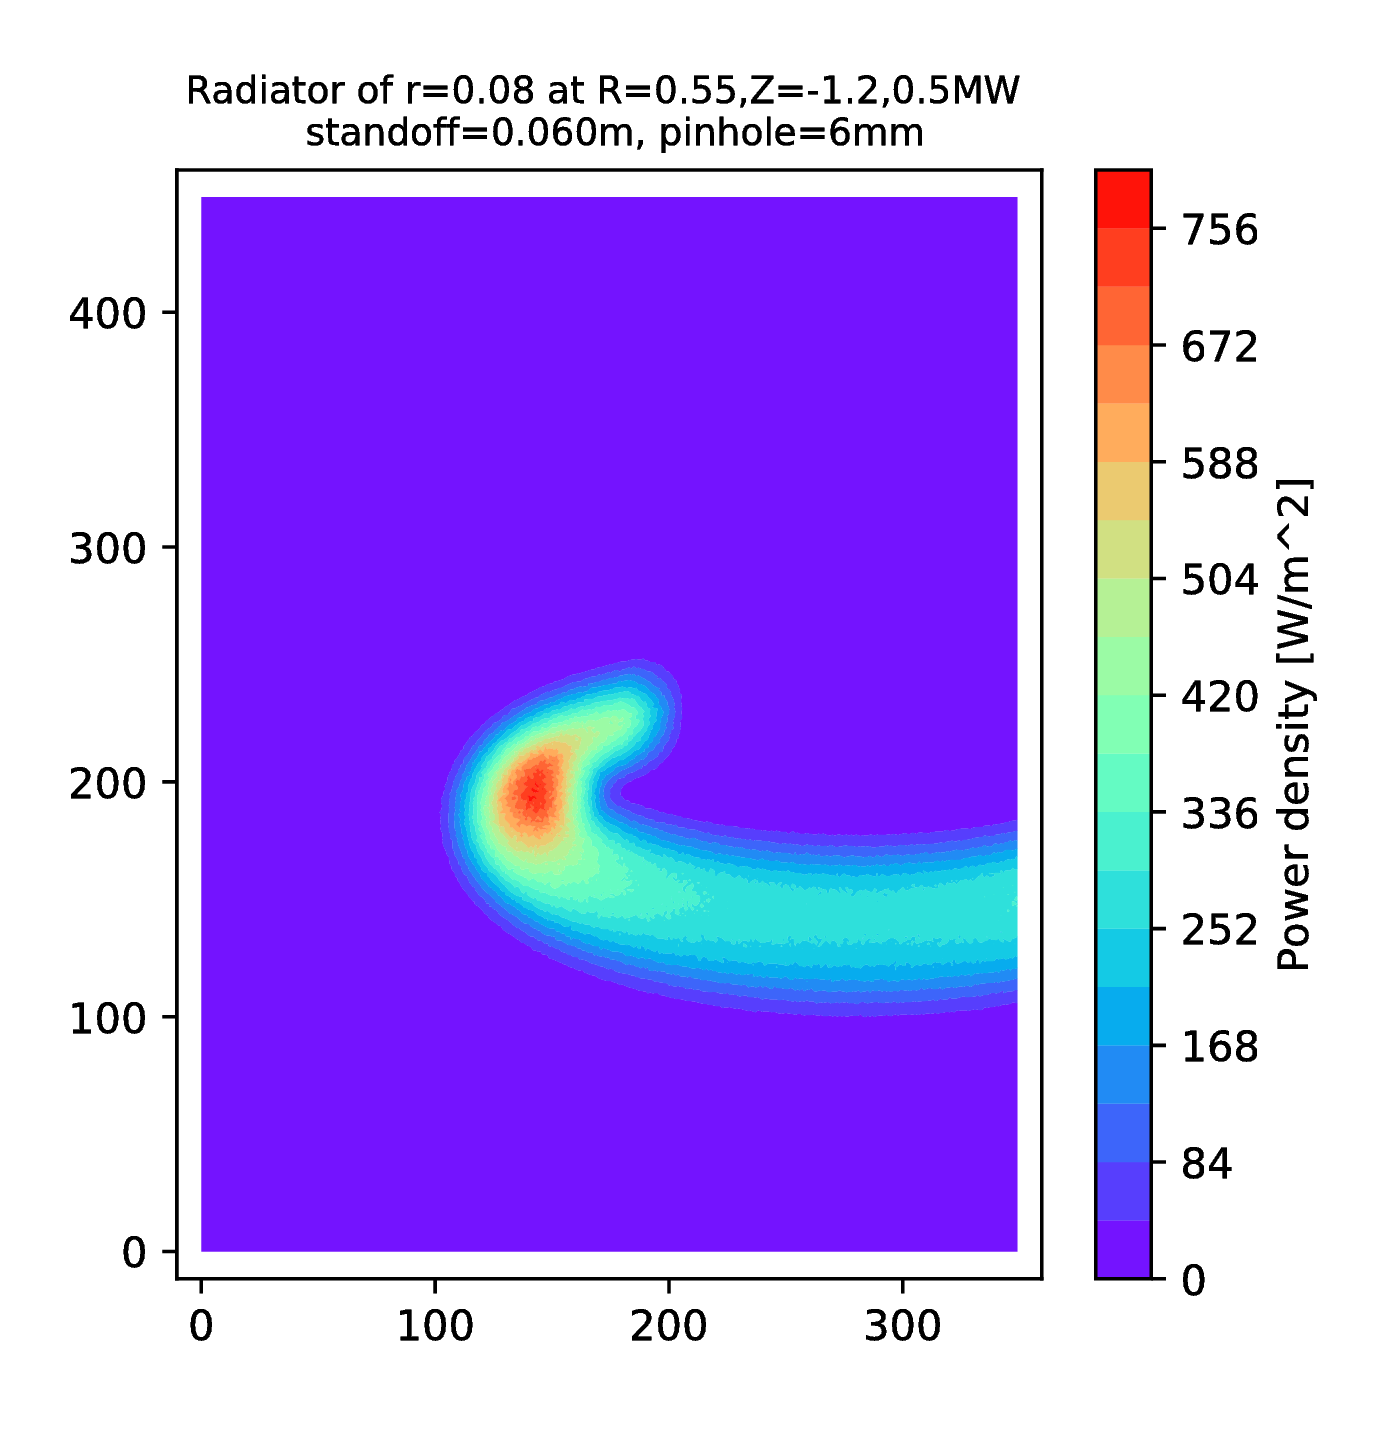
\includegraphics[trim={70 0 125 0},clip,width=\textwidth]{Chapters/appendix1/figs/6_60.png}
         \caption{$6/60$}
         \label{fig:6_60}
     \end{subfigure}
     \hfill
     \begin{subfigure}{0.325\textwidth}
         \centering
         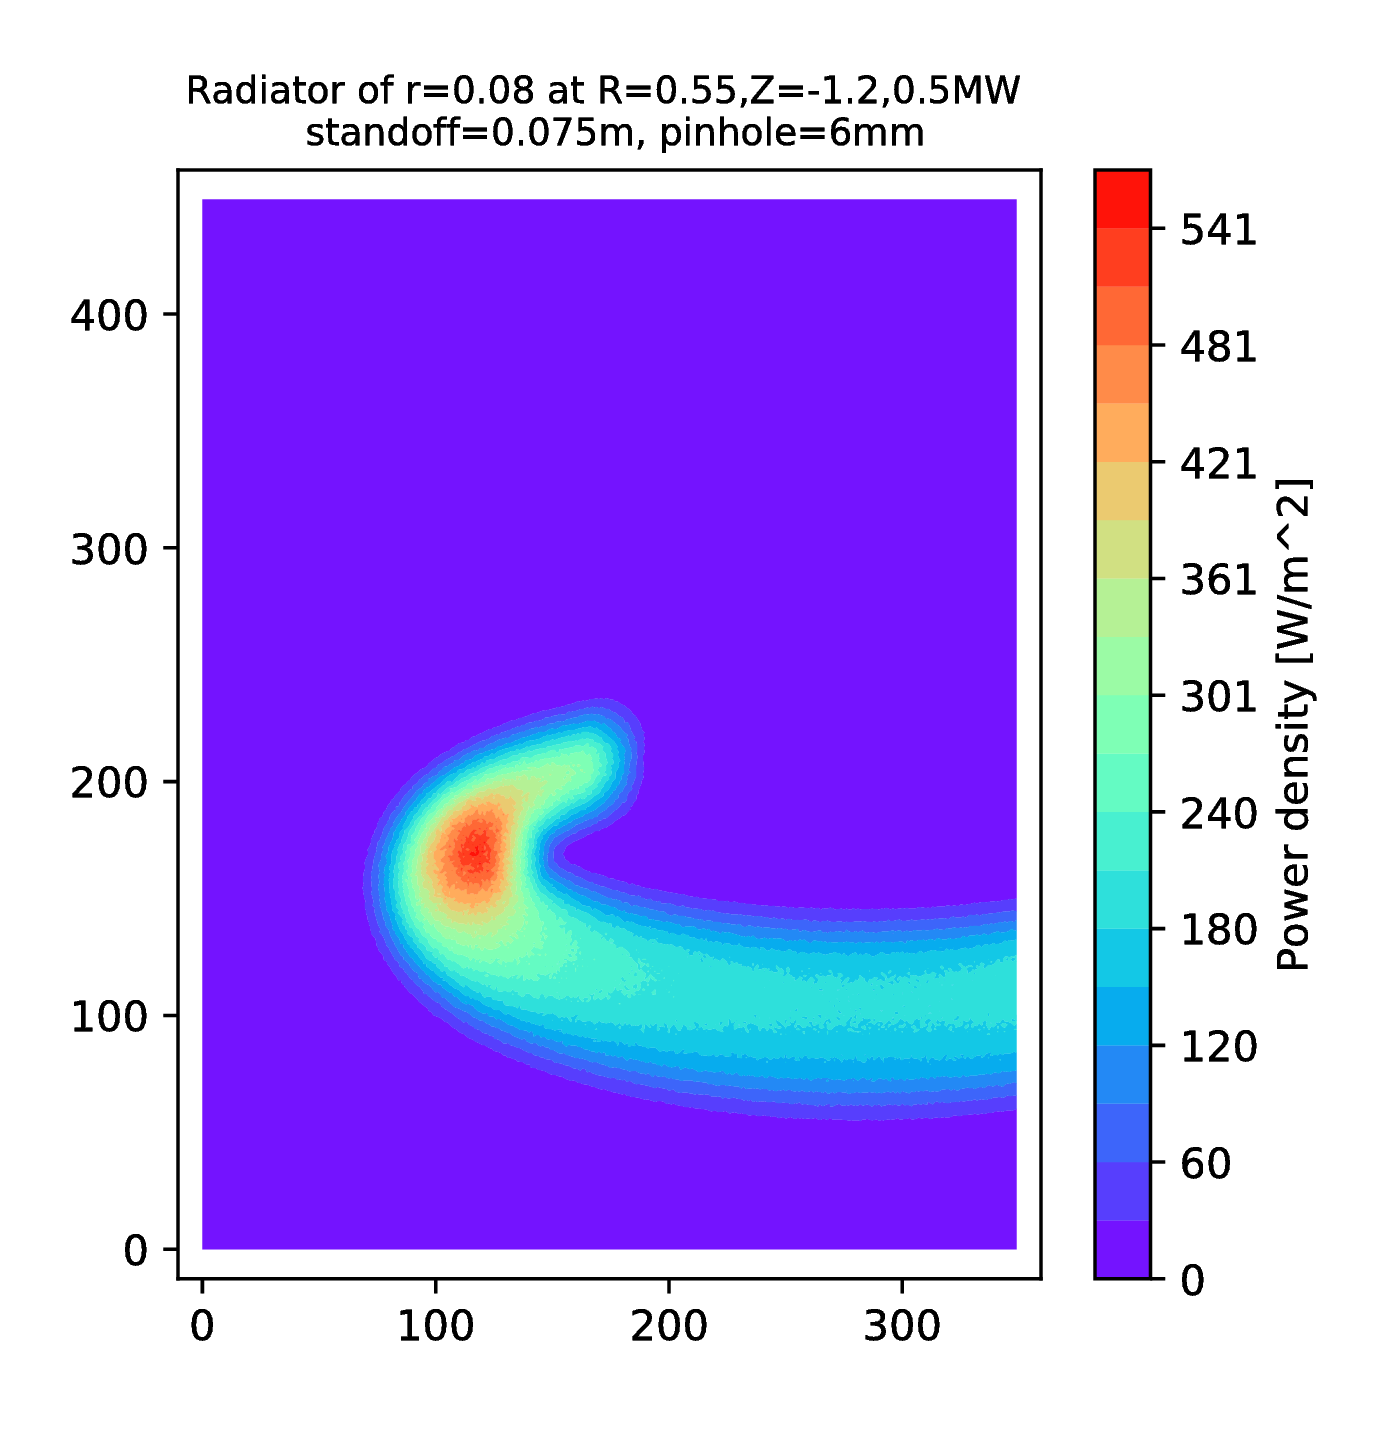
\includegraphics[trim={70 0 0 0},clip,width=\textwidth]{Chapters/appendix1/figs/6_75.png}
         \caption{$6/75$}
         \label{fig:6_75}
     \end{subfigure}
     \begin{subfigure}{0.3\textwidth}
         \centering
         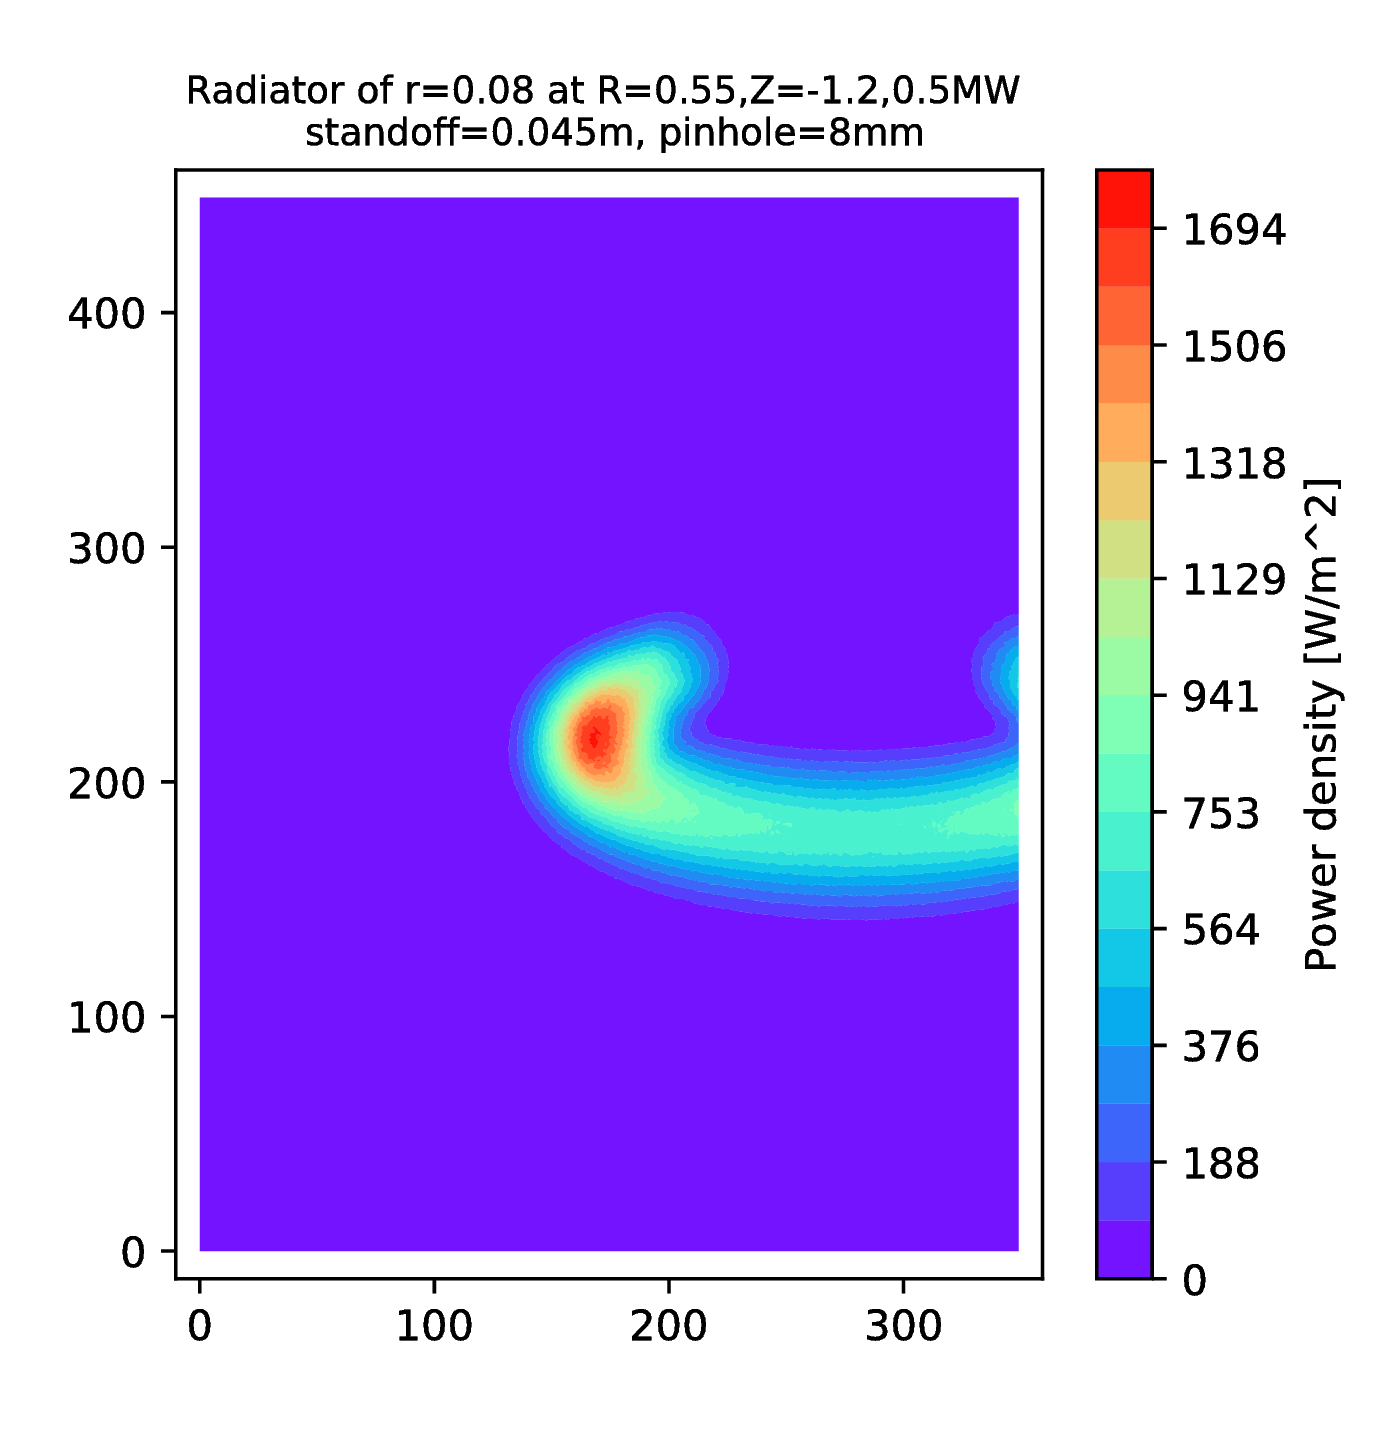
\includegraphics[trim={70 0 110 0},clip,width=\textwidth]{Chapters/appendix1/figs/8_45.png}
         \caption{$8/45$}
         \label{fig:8_45}
     \end{subfigure}
     \hfill
     \begin{subfigure}{0.3\textwidth}
         \centering
         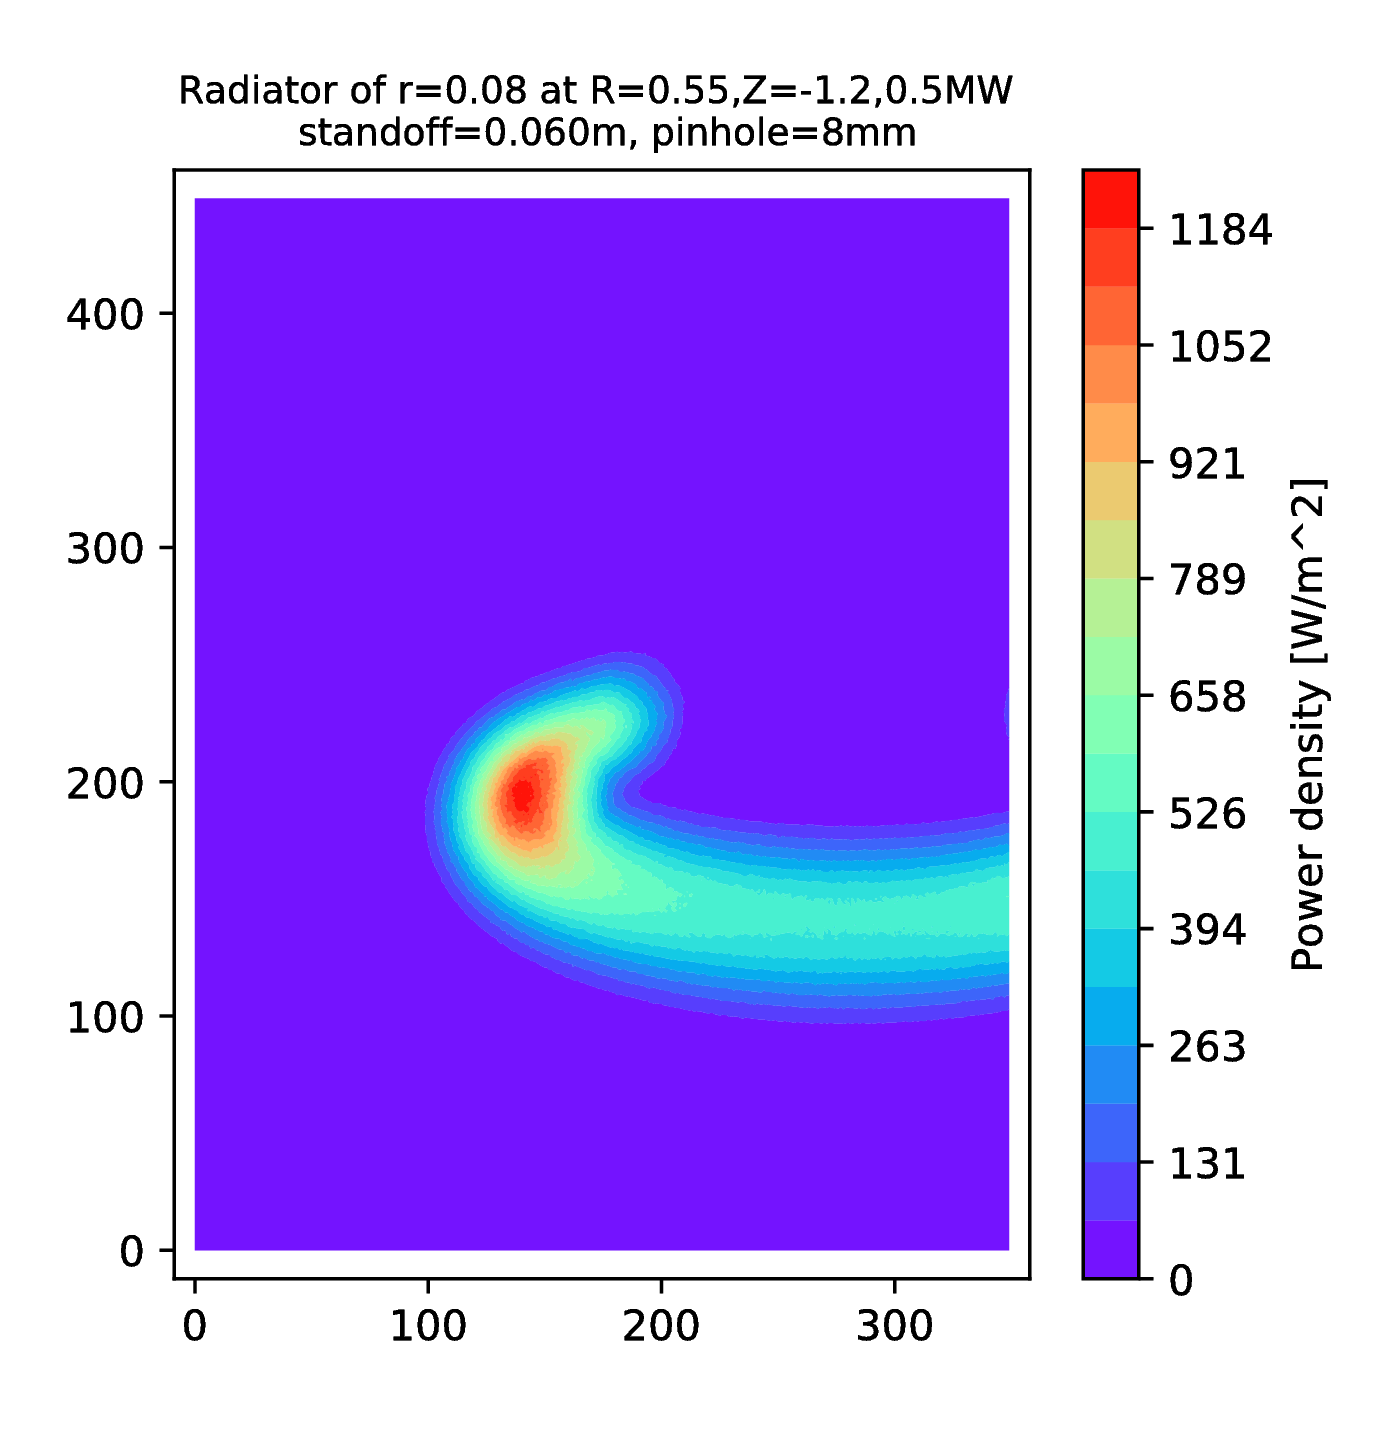
\includegraphics[trim={70 0 110 0},clip,width=\textwidth]{Chapters/appendix1/figs/8_60.png}
         \caption{$8/60$}
         \label{fig:8_60}
     \end{subfigure}
     \hfill
     \begin{subfigure}{0.325\textwidth}
         \centering
         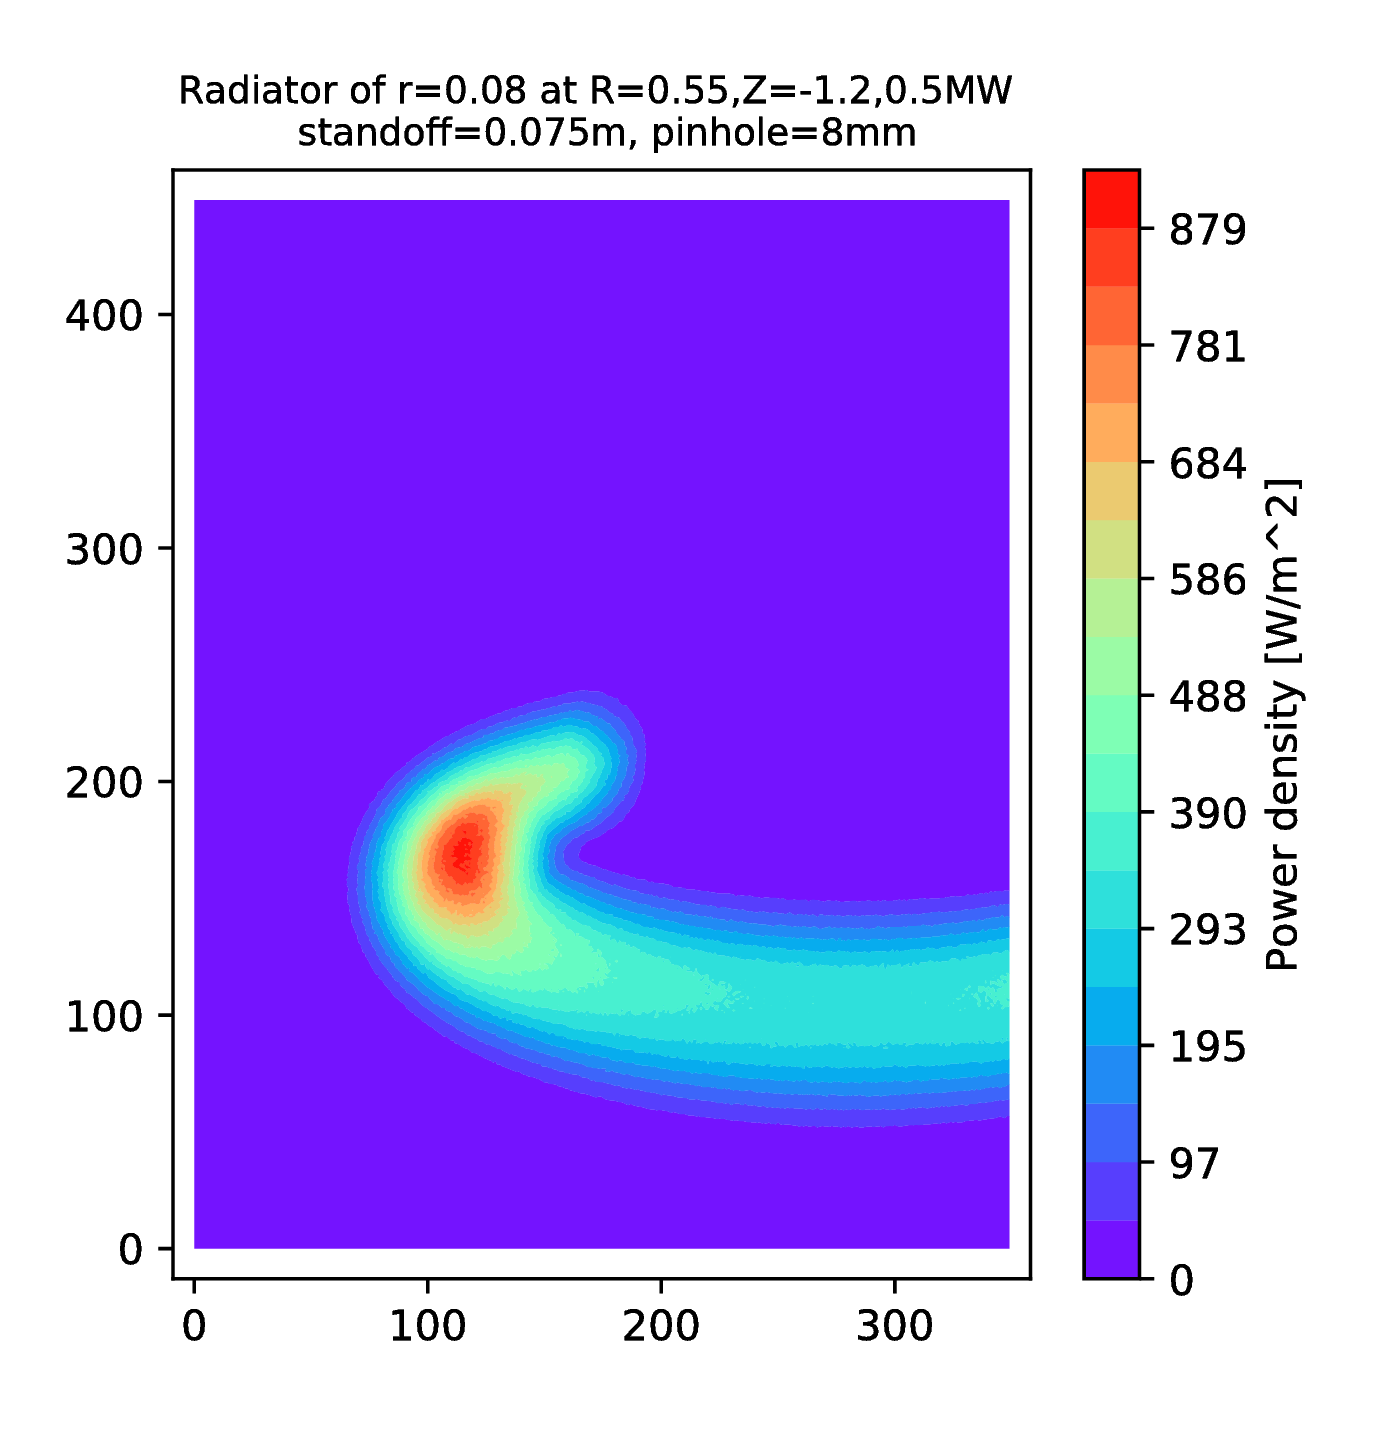
\includegraphics[trim={70 0 0 0},clip,width=\textwidth]{Chapters/appendix1/figs/8_75.png}
         \caption{$8/75$}
         \label{fig:8_75}
     \end{subfigure}

    \caption{Radiation power on the foil from a homogeneous XPR of radius 8cm emitting a total of 0,5MW}
    \label{fig:cherab1}
\end{figure}

The power distribution on the foil was also simulated in the case of a core and divertor region homogeneously filled with emitter. See \autoref{fig:cherab2}.


\begin{figure}
     \centering
     \begin{subfigure}{0.4\textwidth}
         \centering
         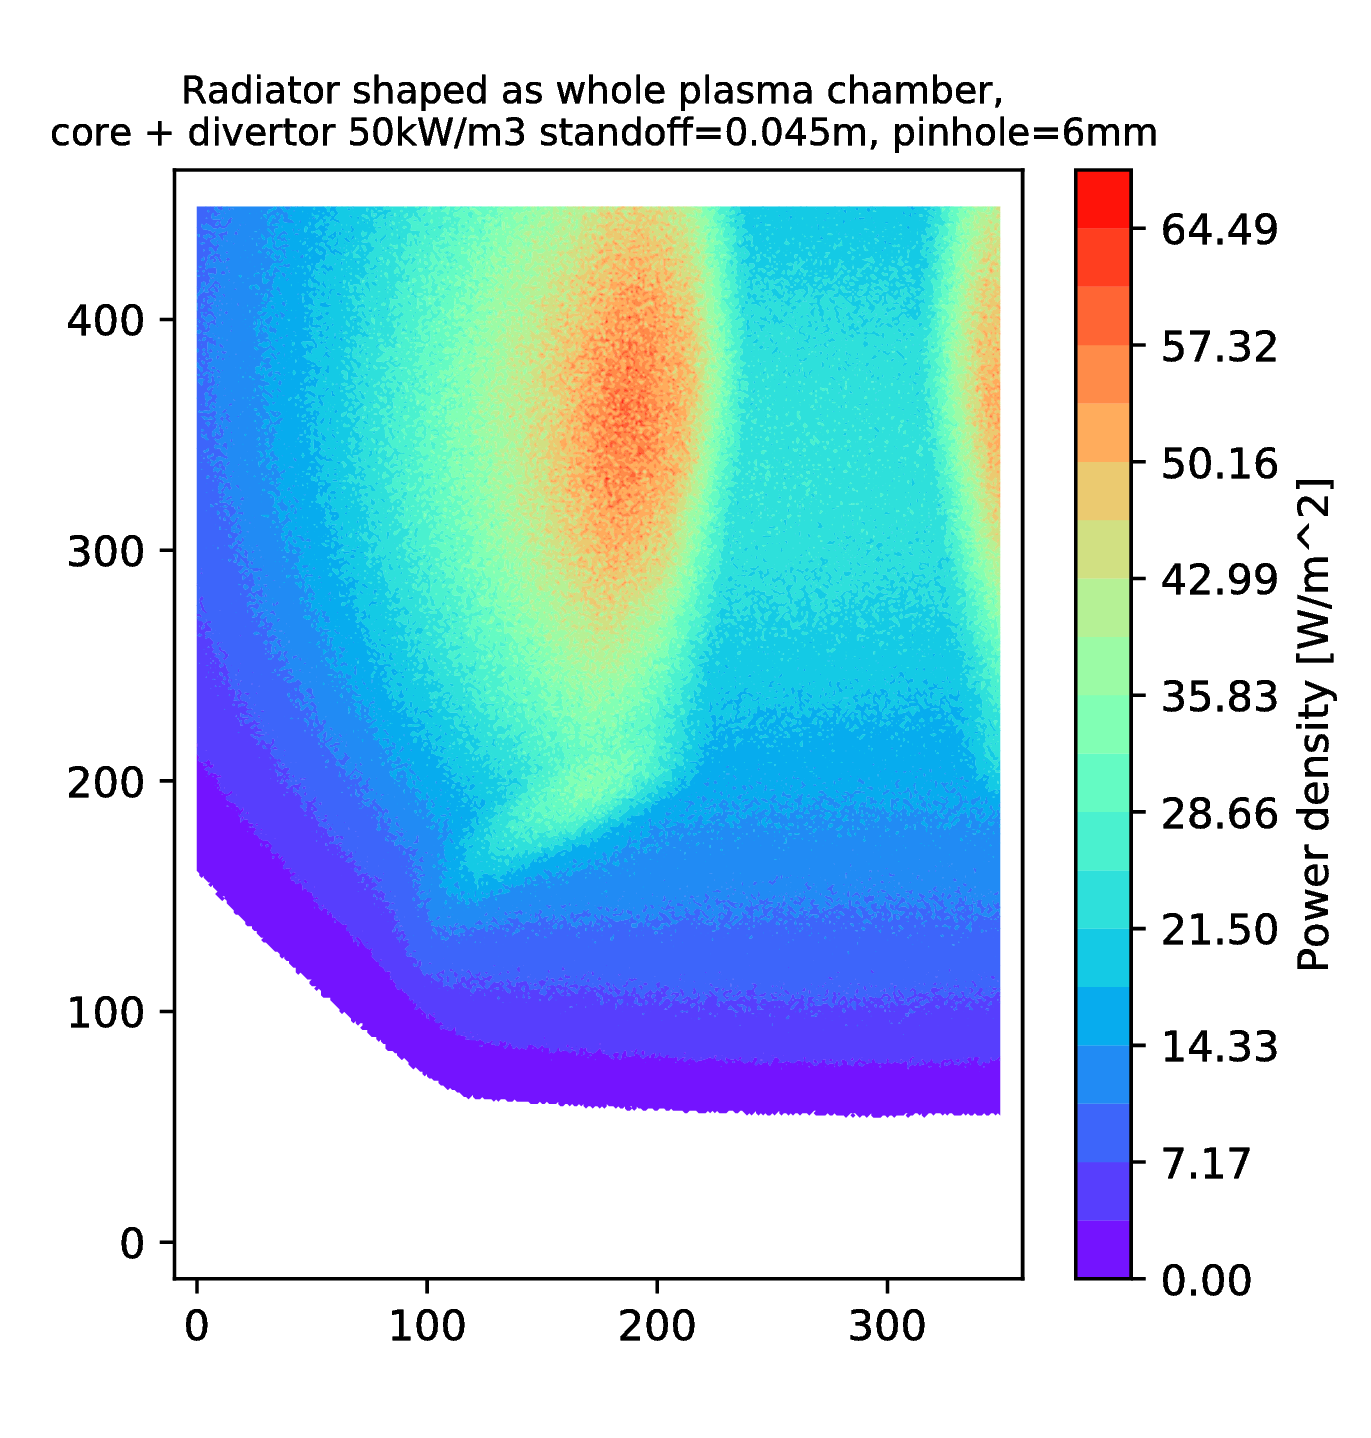
\includegraphics[trim={70 0 0 0},clip,width=\textwidth]{Chapters/appendix1/figs/6_45_all.png}
         \caption{pinhole 6mm/stand-off 45mm}
         \label{fig:6_45_all}
     \end{subfigure}
     \hfill
     \begin{subfigure}{0.50\textwidth}
         \centering
         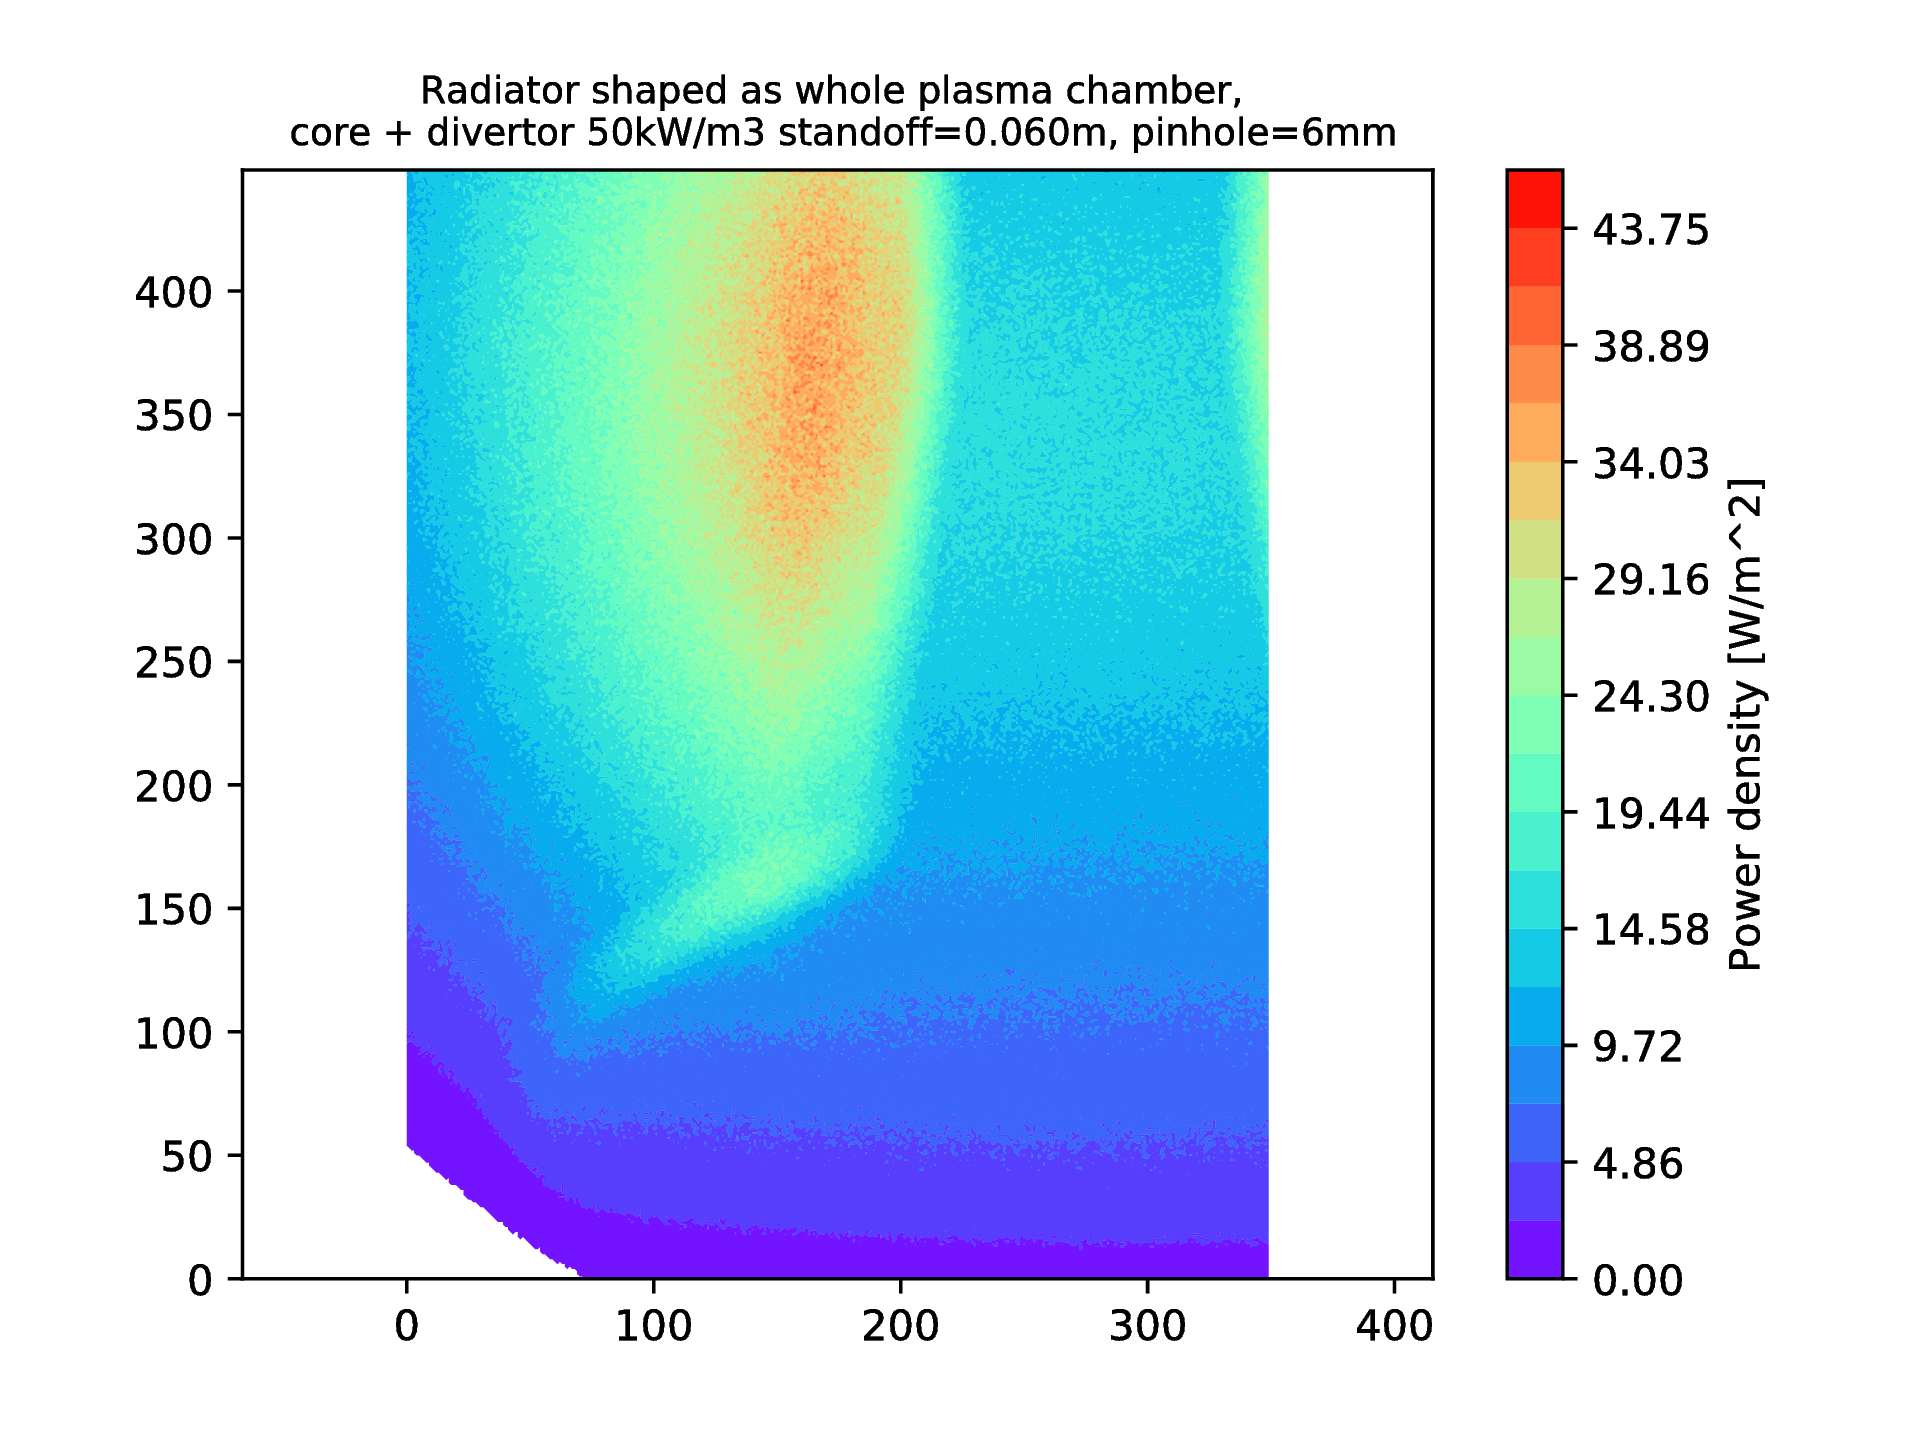
\includegraphics[trim={130 0 150 0},clip,width=\textwidth]{Chapters/appendix1/figs/6_60_all.png}
         \caption{$6/60$}
         \label{fig:6_60_all}
     \end{subfigure}

    \caption{Radiation power on foil with with core and divertor regions emitting homogeneously $50W/m^2$}
    \label{fig:cherab2}
\end{figure}

A bottom left region is clearly visible where no radiation can arrive. This could have been helpful for the prototype phase, because that area could have been used as a reference where the power is zero.
For this reason it has been decided to adopt the stand off 45mm. This allows for an intense enough radiation from the X-point so the smaller pinhole, that allows for a better resolution, 4mm, was selected.

It was later realised that the LOS that enter the super-X chamber have all a similar path through it, causing a large uncertainty on the source of the emissivity there. This can be shown by placing a phantom with known emissivity in the super-x chamber, determining the power on the foil and invert back to the emissivity. The result is shown in \autoref{fig:sxd_bad}.

\begin{figure}
     \centering
     \begin{subfigure}{0.45\textwidth}
         \centering
         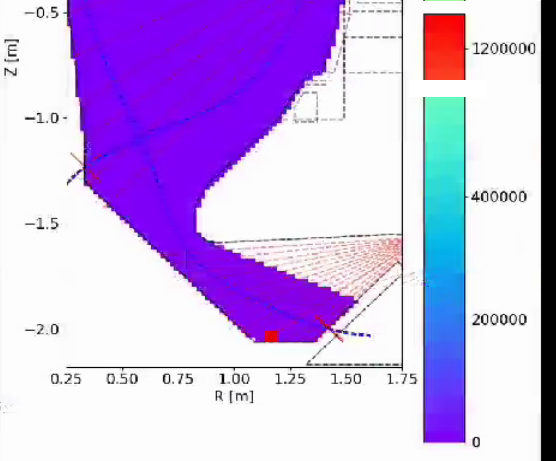
\includegraphics[trim={0 0 30 0},clip,width=\textwidth]{Chapters/appendix1/figs/phantom_sdx.png}
         %\caption{SXD 45239}
         %\label{fig:table45239}
     \end{subfigure}
     \hfill
     \begin{subfigure}{0.45\textwidth}
         \centering
         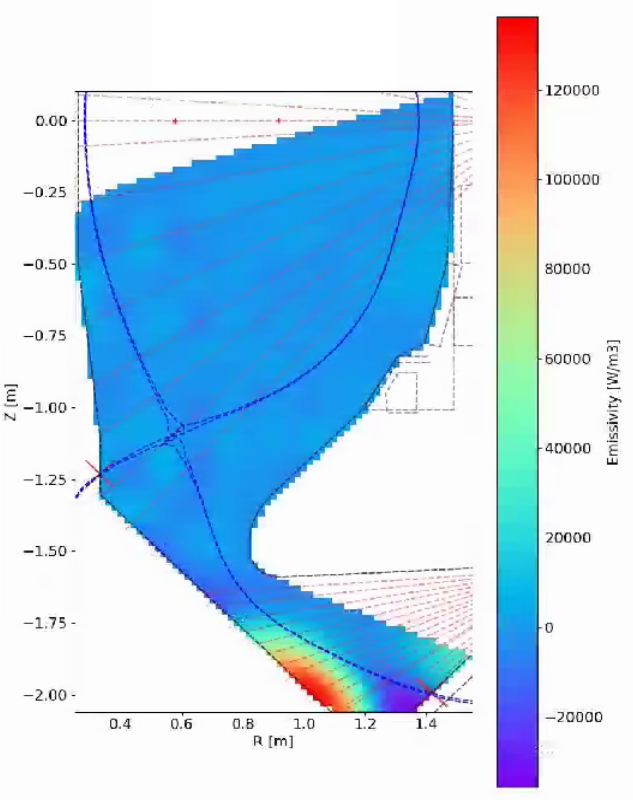
\includegraphics[width=\textwidth]{Chapters/appendix1/figs/inversion_sdx.png}
         %\caption{CD 45401}
         %\label{fig:table45401}
     \end{subfigure}

    \caption{Phantom of radiation localised in the SXD and tomographically inverted emissivity, showing that the present setup is unable to reconstruct detailed emissivity maps of the radiation in the SXD.}
    \label{fig:sxd_bad}
\end{figure}


The inversion routine cannot locate the source of the emission, but the total radiated power in the chamber is still within $\approx 30\%$ of the input.

\subsection{MU02 geometry optimisation}

After the results of the first MASTU campaign it was clear that with appropriate binning the SNR for relatively weak ohmic discharges is large enough (with binning of 14 temporal steps, 7 per digitizer, and 3x3 spatial peak signal on the foil $\approx 40W/m^2$ with uncertainty \hl{$\approx 7W/m^2$}) for high resolution emissivity maps. One negative result is that, because of the small angular difference between the different lines of sights (LOSs) entering the super-x chamber the resolution there is insufficient to reconstruct an emissivity map.
To define the optimal geometry for good SNR two test cases were found:
\begin{itemize}
    \item a ohmic SXD discharge with weak widespread radiation with the purpose of reconstructing the broad characteristics but mostly the total and partial sums of the radiated power. I decided to use 45239 at t=493ms
    \item a conventional high power H-mode discharge from a strong density scan and with x-point radiator, with strong signal, for the purpose of accurately reconstruct the radiation around the x-point. I decided to use 45401 at t=714ms
\end{itemize}

To perform the comparison the emissivity phantoms were calculated for each case with a binning of 14 temporal steps, 7 per camera digitizer, and 3x3 spatial ones with the present geometry. The negative emissivity was set to 0; to recreate a more realistic (field aligned) emissivity profile the emissivity was set to zero at $r>1m$ and $z>-1.5m$ for the 45239 phantom, while at $r>1m$ for 45401. The phantoms created are shown in \autoref{fig:phantoms}. The black dashed lines show the regions that will be used to compare the results.

\begin{figure}
     \centering
     \begin{subfigure}{0.45\textwidth}
         \centering
         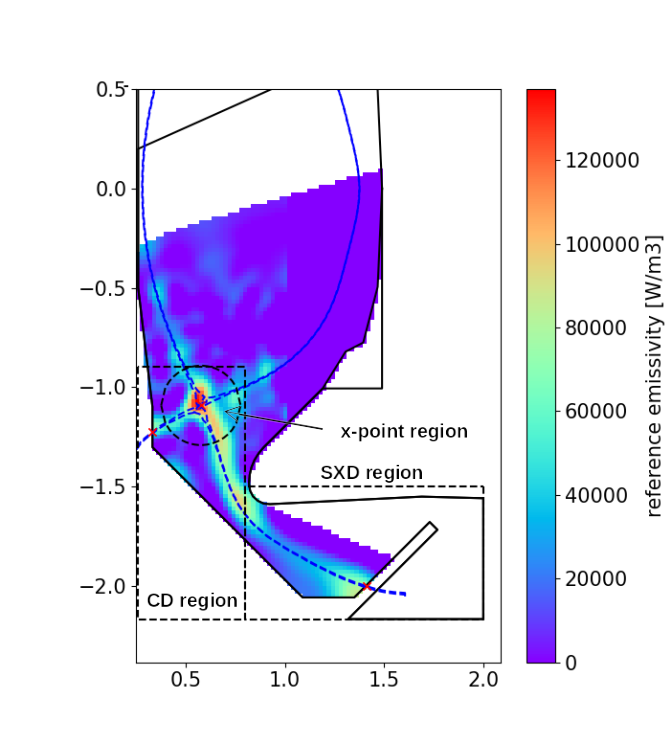
\includegraphics[trim={70 20 0 20},clip,width=\textwidth]{Chapters/appendix1/figs/45239_2.png}
         \caption{SXD 45239}
         \label{fig:45239}
     \end{subfigure}
     \hfill
     \begin{subfigure}{0.45\textwidth}
         \centering
         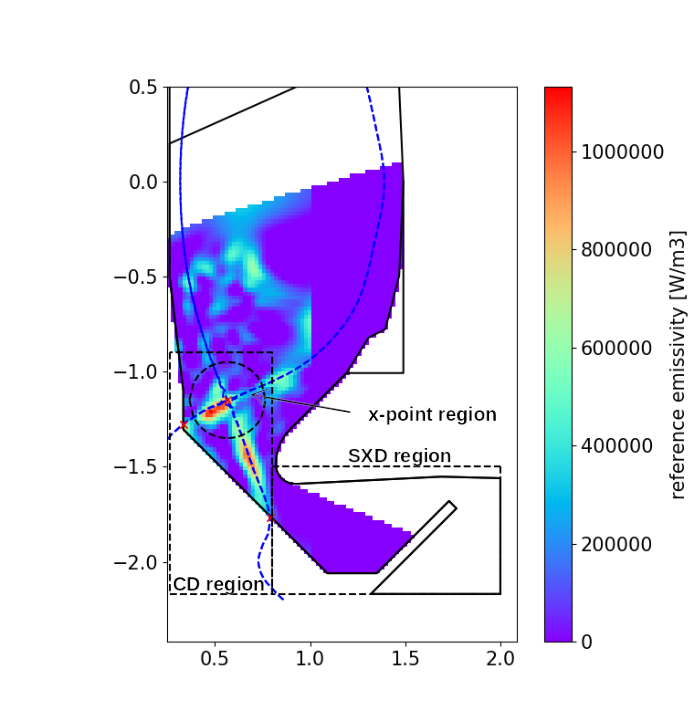
\includegraphics[trim={70 20 0 20},clip,width=\textwidth]{Chapters/appendix1/figs/45401_2.png}
         \caption{CD 45401}
         \label{fig:45401_app}
     \end{subfigure}

    \caption{Phantoms used to compare the effect of different geometries on the tomographic inversion process. Left: shot 45239, 493ms, SXD discharge, emissivity=0 at $r>1m$ and $z>-1.5m$. Right:  shot 45401, 714ms, CD discharge, emissivity=0 at $r>1m$. The dashed lines represent the regions over which the results will be compared.}
    \label{fig:phantoms}
\end{figure}

The configurations investigated are all combinations of 45 and 60mm standoff and 4 and 6mm pinhole. 
For each configuration the geometry matrix is calculated using CHERAB to obtain the power absorbed by the foil. The temperature was then calculated with the same phantom for a number of time steps equal to 4 times the binning and the count noise added. The temperature profile is then binned and the power to the foil is calculated. The tomographic inversion is performed with the intermediate time step to find the new emissivity profile. The profiles are compared to the phantom in terms of local emissivity and integrated power. The results are shown in \autoref{fig:table_mu02}.

\begin{figure}
     \centering
     \begin{subfigure}{0.45\textwidth}
         \centering
         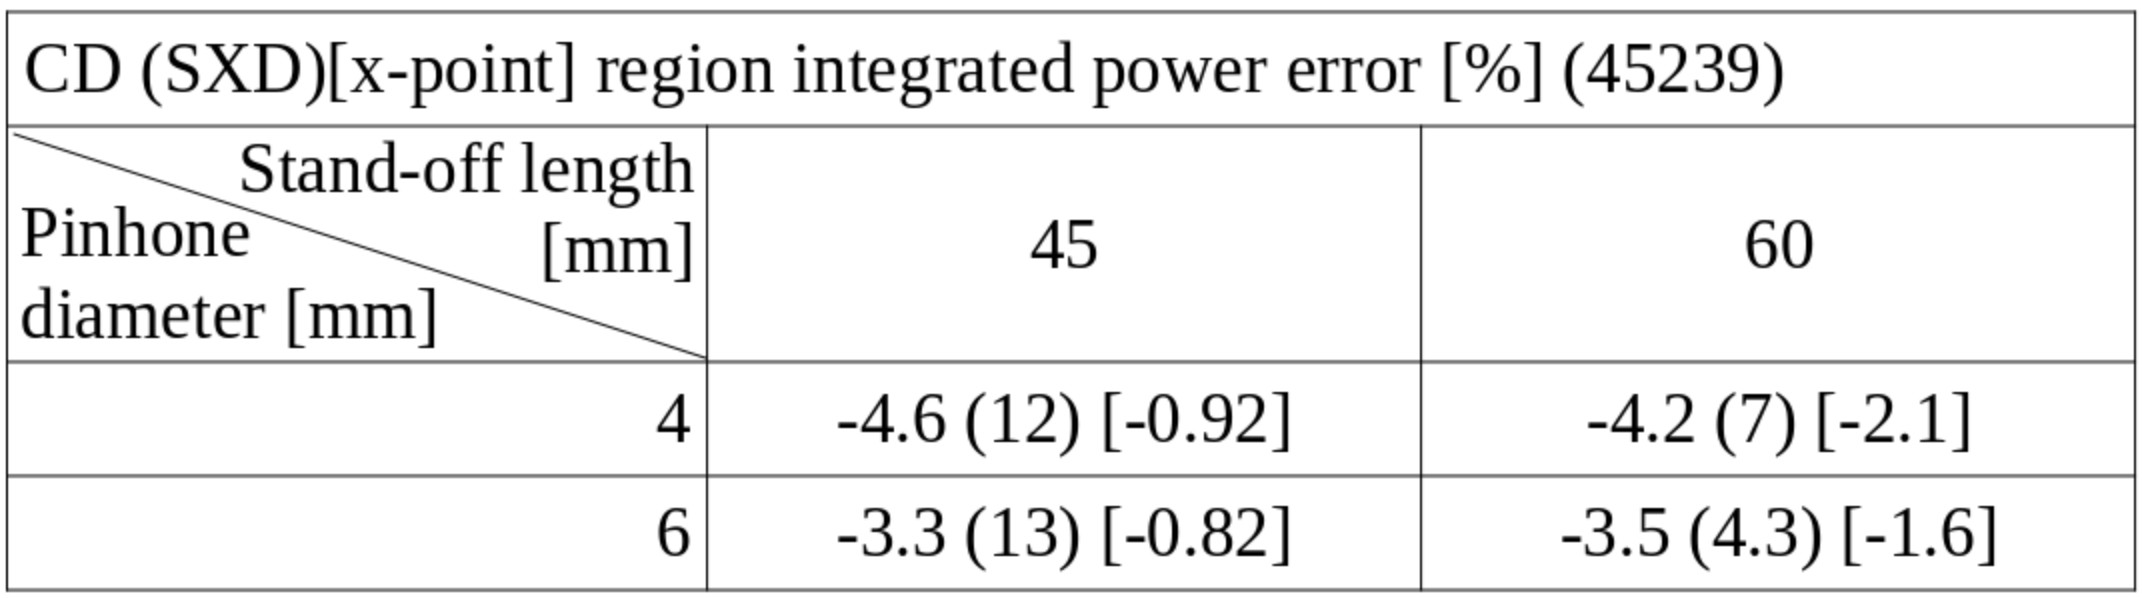
\includegraphics[width=\textwidth]{Chapters/appendix1/figs/table45239.png}
         \caption{SXD 45239}
         \label{fig:table45239}
     \end{subfigure}
     \hfill
     \begin{subfigure}{0.45\textwidth}
         \centering
         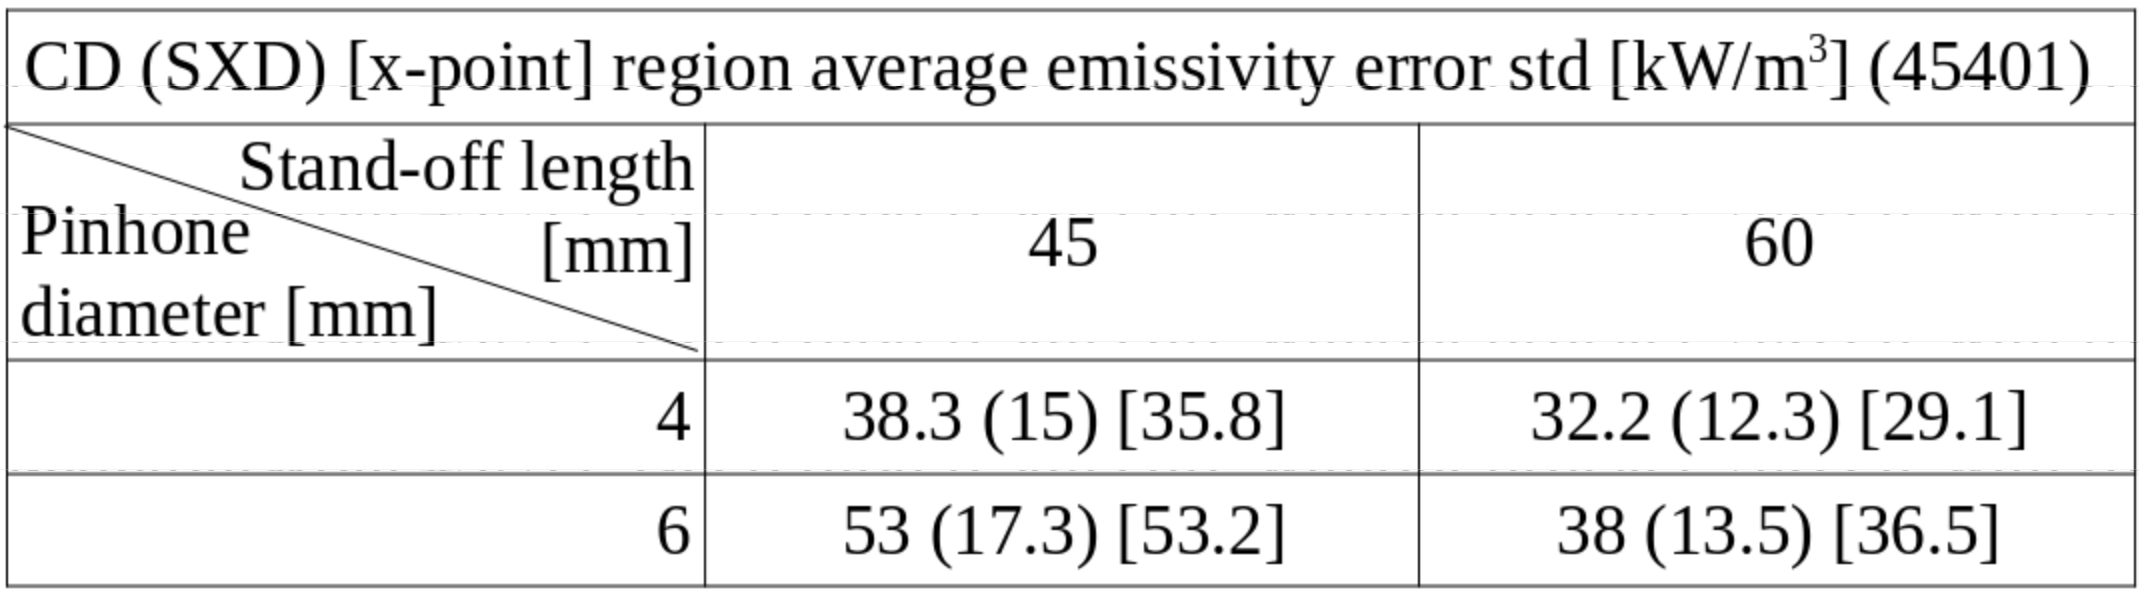
\includegraphics[width=\textwidth]{Chapters/appendix1/figs/table45401.png}
         \caption{CD 45401}
         \label{fig:table45401}
     \end{subfigure}

    \caption{Comparison of the integrated power $\%$ error for all geometric configurations for the SXD phantom from 45239 (a) and of the averaged power error std for all geometric configurations for the CD phantom from 45401 (b). CD region results are without bracket, SXD in with round brackets and x-point ones with square brackets}
    \label{fig:table_mu02}
\end{figure}

A larger pinhole allows a more precise accounting of the integrated power. Given the present SNR though, the improvement is minor. This is even more true considering that in MU02 the discharges are expected to be more energetic, with beam power even in L-mode. The power accounting in the SXD also improves with a longer stand-off.
The 60mm stand-off 4mm pinhole diameter configuration yields the better performance in terms of resolution around the x-point with strong signal. For high SNR additional LOSs count more than an even stronger signal.

Regarding the loss of spatial resolution in the SXD the stonger the signal the better. For larger pinhole the reconstructed radiation is more localised but still elongated along the LOS. Considering the design of IRVB aimed at a high resolution around the x-point and not the SXD, this is considered less important. It will be important to remember that the data inside the SXD is useful for integrated measurements rather than profiles.
With these consideration it was decided to adopt the 4mm diameter pinhole and 60mm long stand-off. It is the solution that causes the lower signal strength, but it is still deemed sufficient.

\section{IRVB calibration}\label{IRVBcalibration}
\subsection{Temperature}

In order to test every pixel of the camera with the limited size of the BB source available the source was taken as close as possible to the view port making it out of focus. This could be done as the whole surface of the BB cavity emits the same amount of radiation isotropically. This was verified by performing 3 separate calibrations: camera and BB source as close as possible ($\approx 10cm$, some room was necessary for the window in between the two), as far as possible (with the whole field of view still inside the source, $\approx 18cm$) and with the source in focus ($\approx 65.7cm$). It was found that the effect on the a1 coefficient is negligible.
The geometry of the calibration is represented in \autoref{fig:BBcalib} .

\begin{figure}
	\centering
	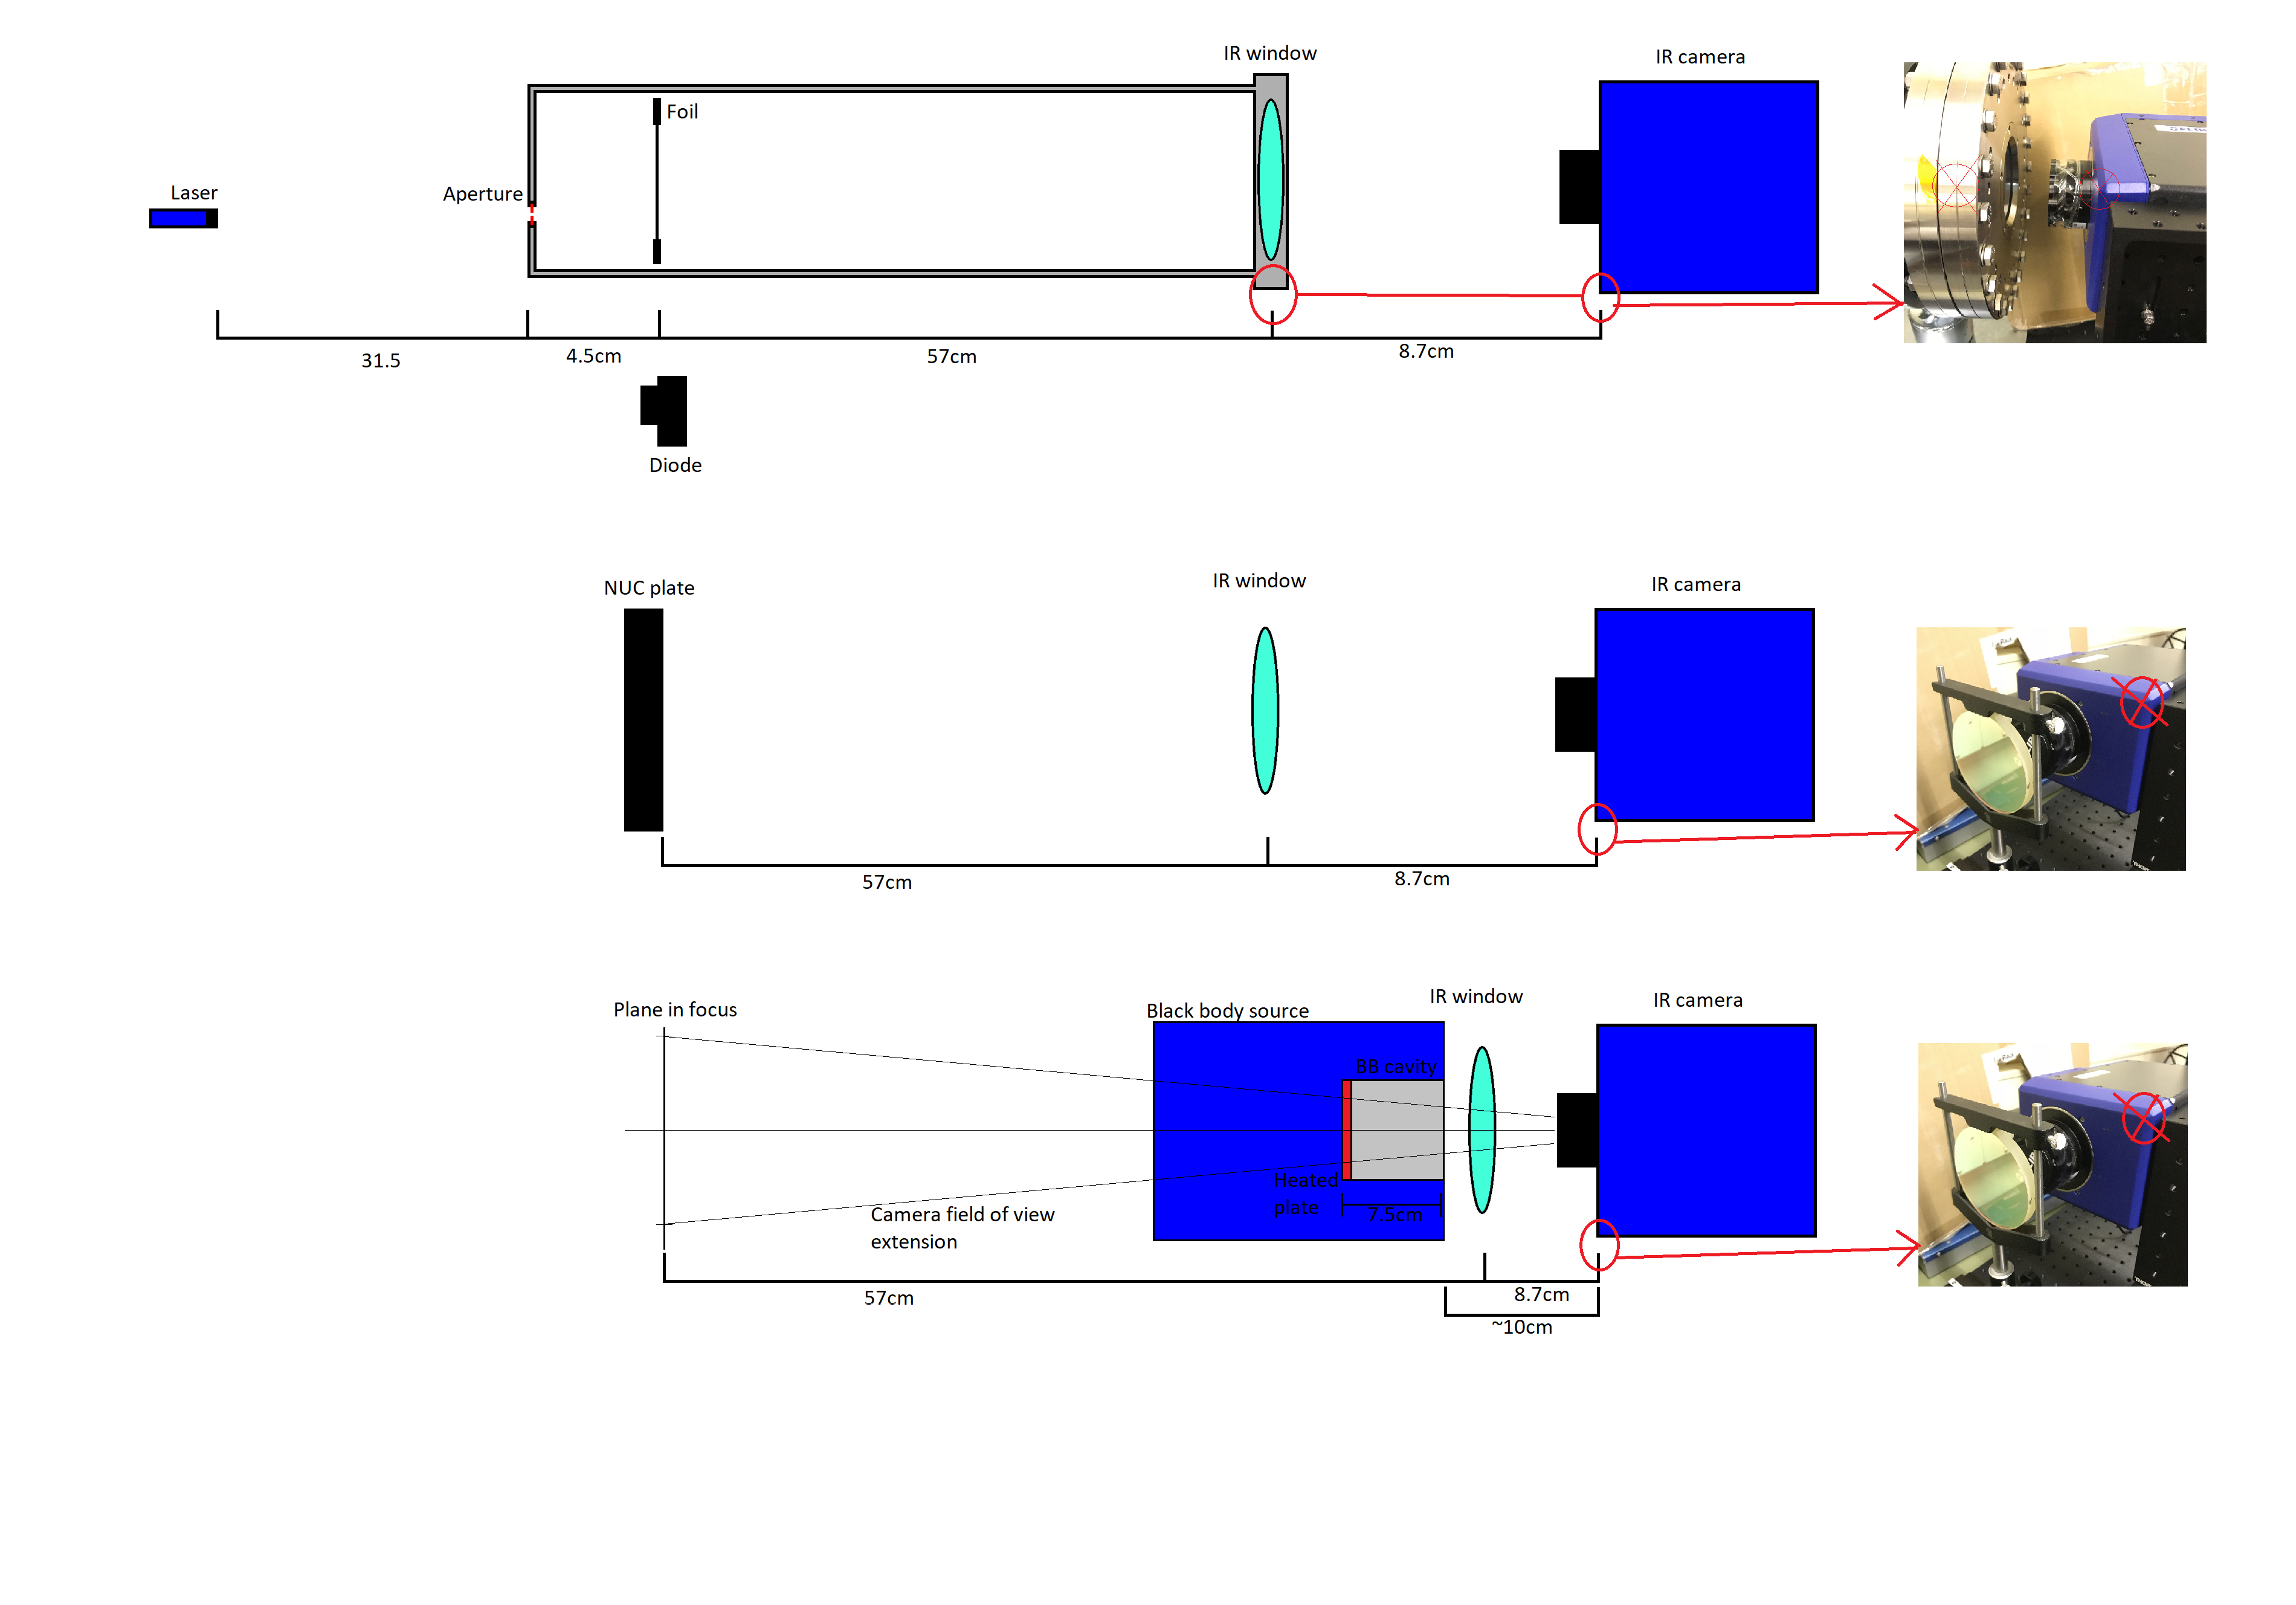
\includegraphics[trim={800 300 0 1200},clip,width=\linewidth]{Chapters/appendix1/figs/calib_schematics.png}
	\caption{Schematic of the calibration setup. The plane in focus correspond to the distance at which the IRVB foil is. The window is at the same distance from the camera as when installed on MASTU}
	\label{fig:BBcalib}
\end{figure}

The results of the calibration are shown in \autoref{fig:BBcaliba1}, \ref{fig:BBcaliba3} and \ref{fig:BBcaliba1a3SNR}. As expected, most of the flat offset is in $a_2$ while only a minor component in $a_4$. The $a_1$ coefficient seems completely not effected by the narcissus effect. Conversely the corrective factor $a_3$ seems dominated by it, while still being $>0.95$ across the thole field of view with a relative variation less then half of $a_1$. The $a_2$ and $a_4$ coefficients are irrelevant as are not used in the temperature and power calculations.

\begin{figure}
	\centering
	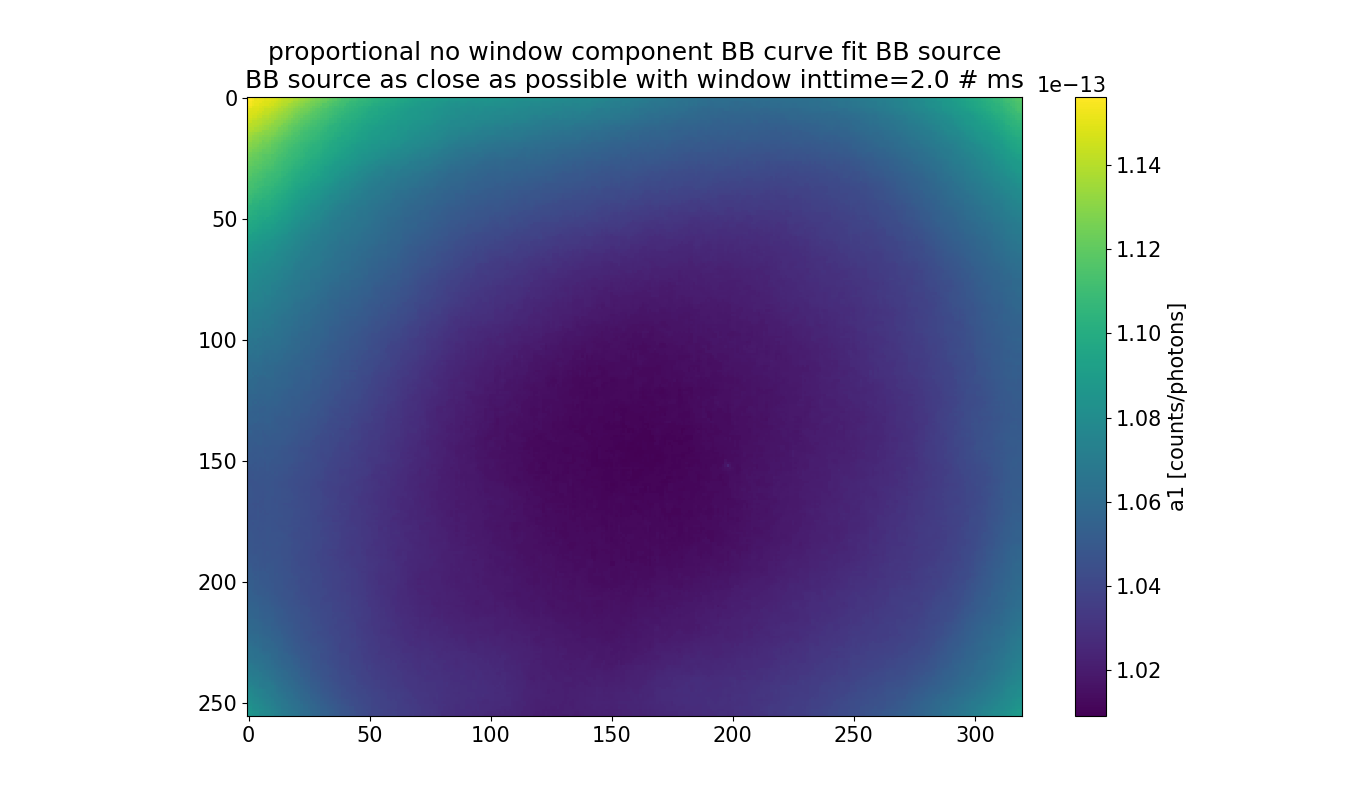
\includegraphics[width=\linewidth]{Chapters/appendix1/figs/calib_a1.png}
	\caption{$a_1$ coefficient obtained via calibration with BB source}
	\label{fig:BBcaliba1}
\end{figure}
\begin{figure}
	\centering
	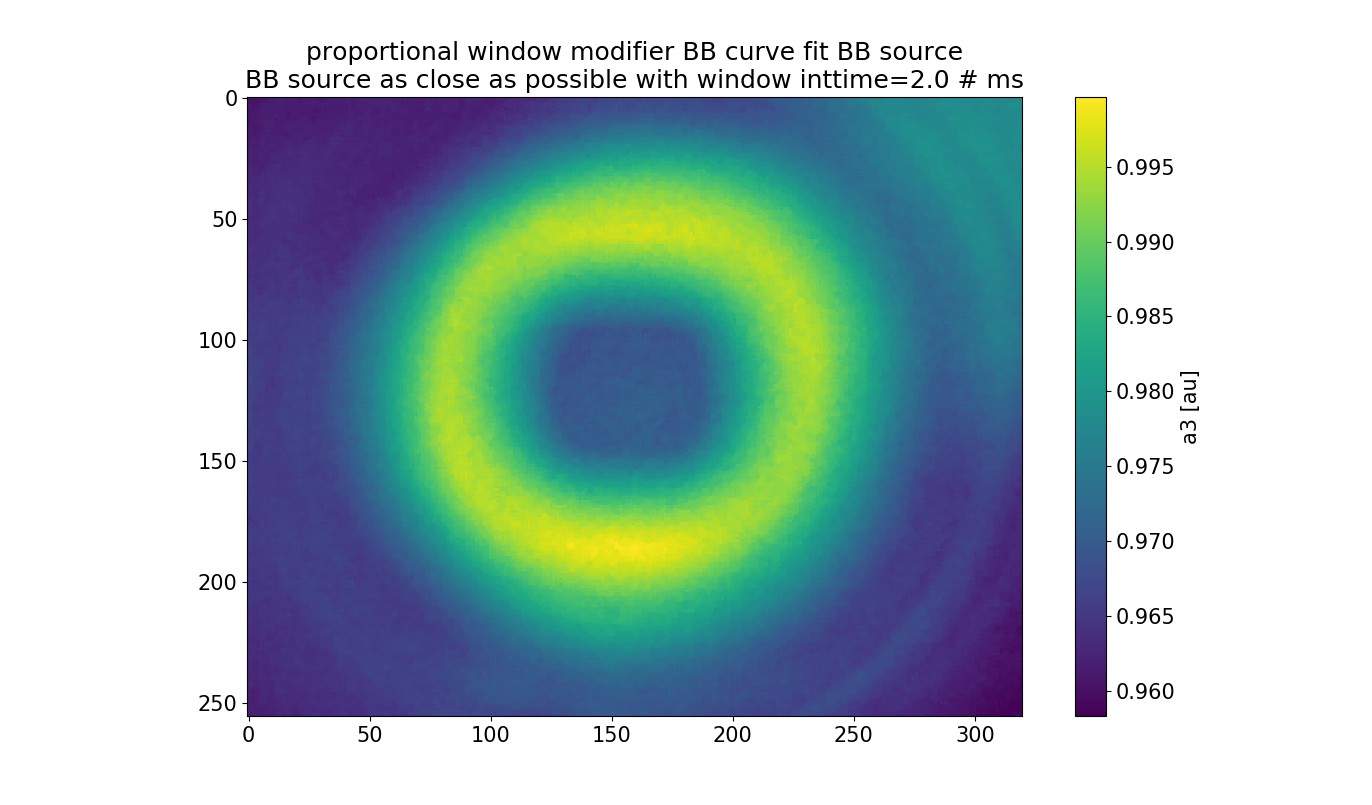
\includegraphics[width=\linewidth]{Chapters/appendix1/figs/calib_a3.png}
	\caption{$a_3$ coefficient obtained via calibration with BB source}
	\label{fig:BBcaliba3}
\end{figure}
\begin{figure}
	\centering
	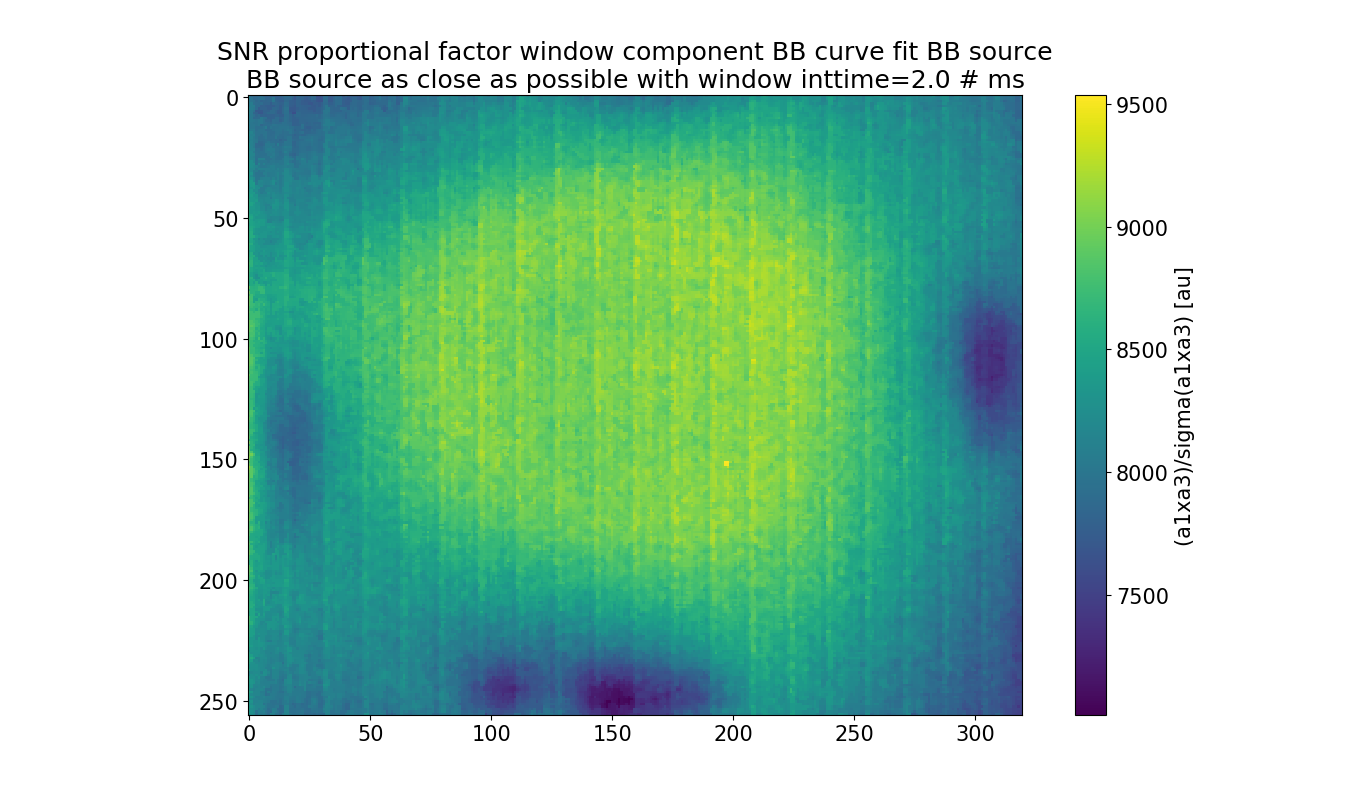
\includegraphics[width=\linewidth]{Chapters/appendix1/figs/calib_a1a3SNR.png}
	\caption{$a_1 a_3 / \sigma_{a_1 a_3}$ obtained via calibration with BB source}
	\label{fig:BBcaliba1a3SNR}
\end{figure}

An alternative method for temperature calibration was also tested. A Solfadir non uniformity calibration (NUC) plate, was pre-heated or cooled to a set temperature and let transition to room temperature. The NUC plate is large enough to fill the entire field of view and being in focus. Its surface is such to have an emissivity close to 1. The temperature of the plate is recorded and various samples are collected with the IR camera while the plate temperature approaches ambient. The data is then fit with a low order polynomial curve. This procedure introduces 2 issues:
\begin{itemize}
    \item the NUC plate is cooled or heated by the air via conduction, convection and BB radiation. This causes the plate to not have a homogeneous temperature. During these tests it was estimated that the temperature non uniformity reached ~0.4K, and up to 0.1K in the -5/+5K temperature range around room temperature. This is of course not ideal for the IRVB, as the measurement of the power absorbed by the foil relies on very small temperature differences
    \item The temperature/counts correlation does not rely on to a physical model, but it is a simple polynomial that will try to match the real physical dependency behind the IR measurements. The physics of a BB source is fairly simple, and the only factors are the wavelength range and emissivity. The camera could potentially have a different sensitivity for different photon energy, but this is usually neglected given the small wavelength range allowed by the filter ($2,5-5\mu m$).
\end{itemize}
For these reasons this method was later abandoned.

\subsection{Foil characteristics}
To calibrate the foil $t_f$ thickness, $\kappa$ thermal diffusivity and $\varepsilon$ black body emissivity must be determined. A set of spatially resolved parameters was supplied together with the foil of which the average correspond to $\epsilon=0.85+/-0.04, t_f=1.29+/-0.17 \mu m$ with nominal platinum $\kappa=2.5\;10^{-5}m^2/s$. There are different ways to find the foil parameters, see as reference \cite{Itomi2014,Cernuschi2001,Mukai2016}. The method of choice was to shine a pulsed laser \hl{(make and model)} of known intensity to the foil through the pinhole while the whole tube was maintained in the vacuum. The temperature of the foil was monitored with the IR camera. The laser intensity, frequency and focus was varied: with slow pulses the time variation component tends to become irrelevant such that only black body and diffusion remain. With a defocused laser the temperature increase is low and the spatial distribution slowly varying, leaving the black body radiation as the major contributor. with a fast pulsed laser the time dependent component is dominant. The power on the foil determined with \autoref{eq:heat2d} is then compared to the known input. The transmission of the vacuum window on the laser side was measured at $93.3\%$ and taken into account. The fit returned the properties: $\epsilon=1, t_f=2.05 \mu m, \kappa=1.03\;10^{-5}m^2/s$. These values were assumed uniform and used in processing MASTU data, with as uncertainties the variability from the spatially resolved parameters.
\subsection{counts oscillation suppression}
not sure if this is necessary
\subsection{geometry matrix: CHERAB}
not sure if this is necessary